\documentclass{myBeamer}

%% Title page
\title{Ordinary Differential Equations}
\subtitle{as an alternative to agent-based modelling}
\author{eX Modelo school}
\date{June 26, 2019}
\institute{
\includegraphics[scale=1.5]{figures/logos/openmole.png}}


\begin{document}

\begin{frame}[plain]
	\titlepage
\end{frame}
\addtocounter{framenumber}{-1}

\AtBeginSection[]
{
	\frame{
		\sectionpage
	}
	\addtocounter{framenumber}{-1}
}


\section{ODE systems}

\sframe{The ODE framework}{
	$\rightarrow$ widely used to model transmission phenomena\\
	
	\bigskip
	
	\begin{center}
	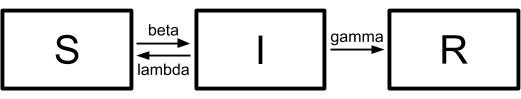
\includegraphics[width=.75\textwidth]{figures/SIR.jpg}
	\end{center}
	
	\bigskip
	
	\begin{itemize}
		\item population split into compartments
		\item system of ordinary differential equations
	\end{itemize}
}


\sframe{SIR model}{
	\begin{center}
	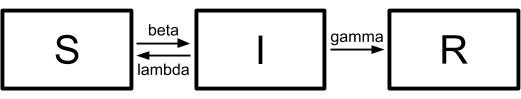
\includegraphics[width=.75\textwidth]{figures/SIR.jpg}\\
		
	\begin{eqnarray*}
	\left\{
	\begin{array}{lcl}
		\dv{S}{t}  & = &  -\beta S + \lambda I \\
		\tmspace{1mu}&& \\
		\dv{I}{t} & = & \beta S - (\lambda + \gamma)I \\
		\tmspace{1mu}&& \\
		\dv{R}{t} & = & \gamma I
	\end{array}
	\right.
	\end{eqnarray*}
	\end{center}
}


\sframe{SIR model dynamics}{
	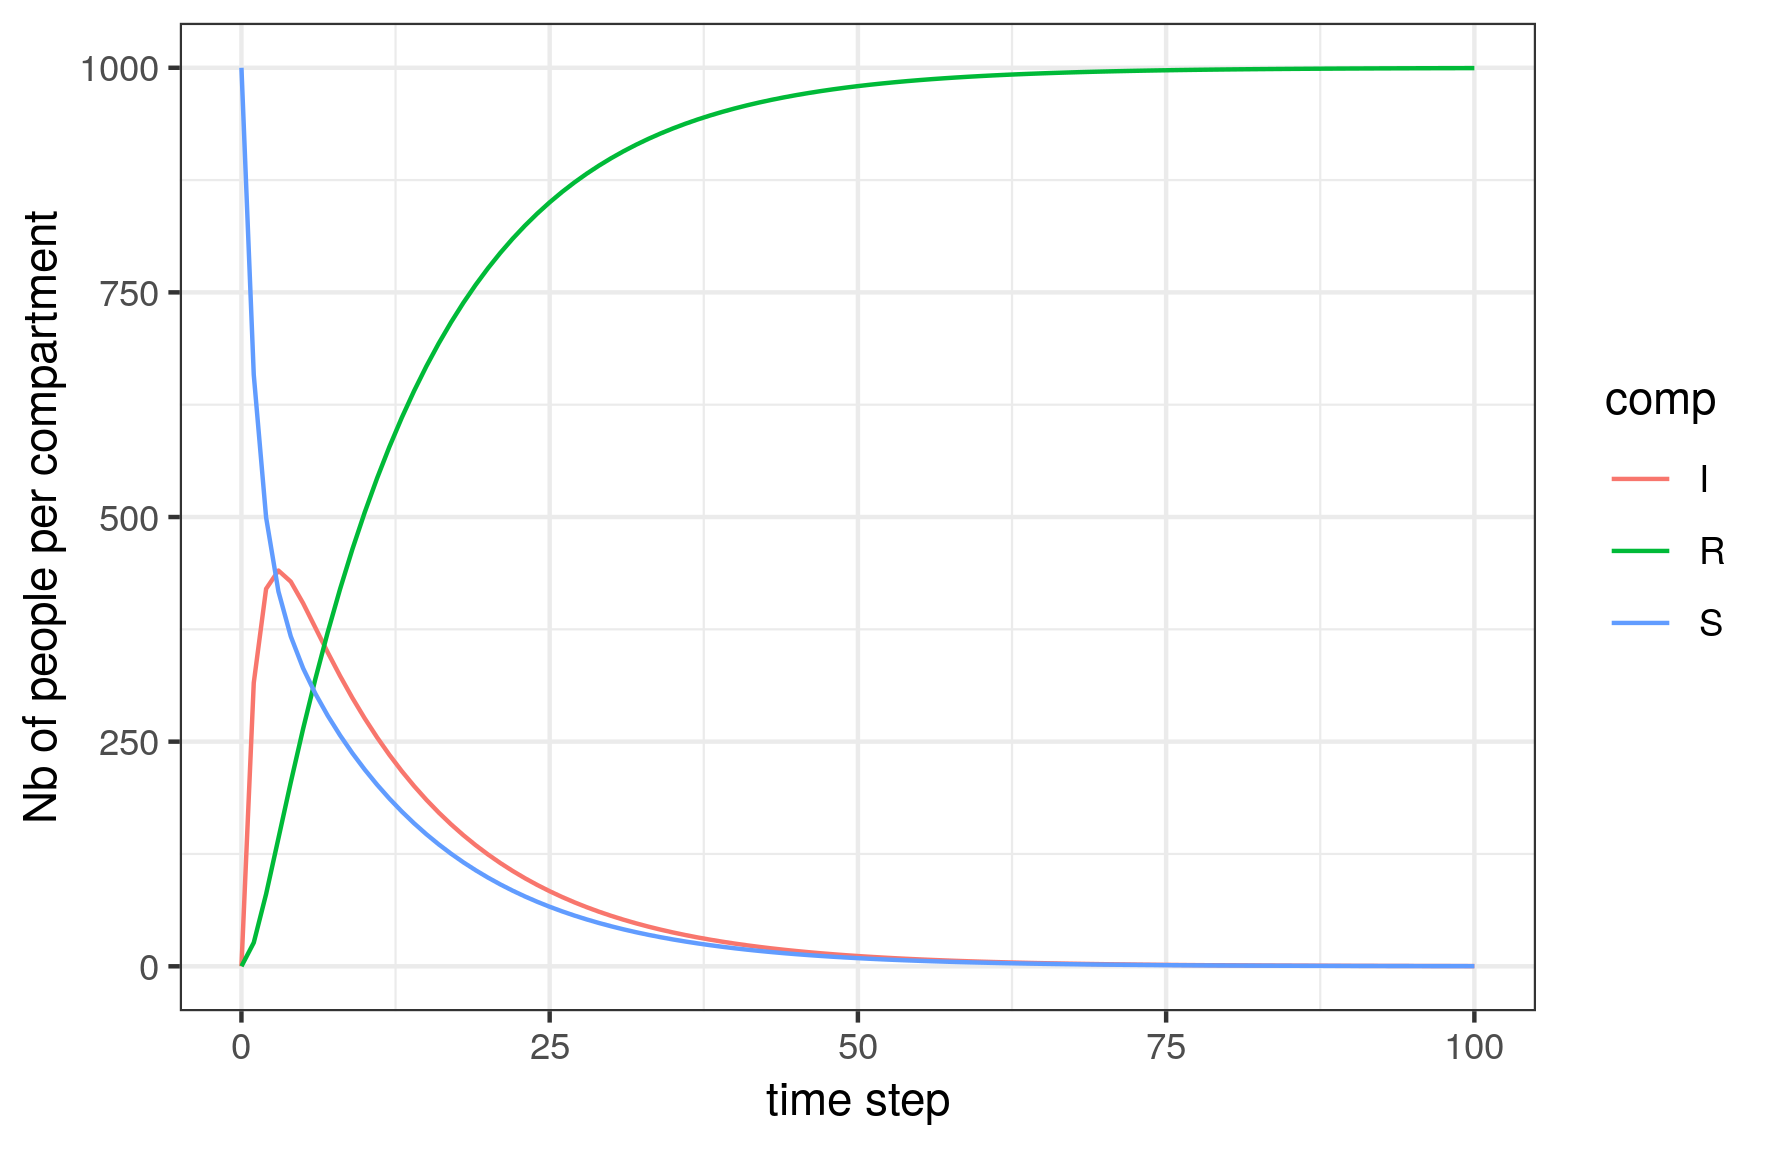
\includegraphics[width=\textwidth]{figures/SIRdynamics.png}
}


\sframe{ODE vs ABM}{
	\begin{table}
 	\begin{tabular}{ll}
 		\thead{\head{ODE}} & \thead{\head{ABM}} \\
		Equation-based & Individual-based \\
		Generic mechanisms & Precise mechanisms \\
		Population scale & Individual scale \\
		Needs less resources & Computationally  expensive
  	\end{tabular}
  	\end{table}
}


\section{A Zombie situation}

\sframe{An ODE model for our Zombie problem}{
	\head{How could we model the Zombie invasion?}
	
	\begin{itemize}
		\item Which mechanisms?
		\item Which parameters?
	\end{itemize}
	
	\bigskip
	
	\visible<2>{
	\head{How can we assess our model's ability to reproduce the real data?}
	
	\begin{itemize}
		\item Which metrics?
		\item Which fitness function?
	\end{itemize}
	}
}


\sframe{A very simple ODE model}{
	\begin{center}
	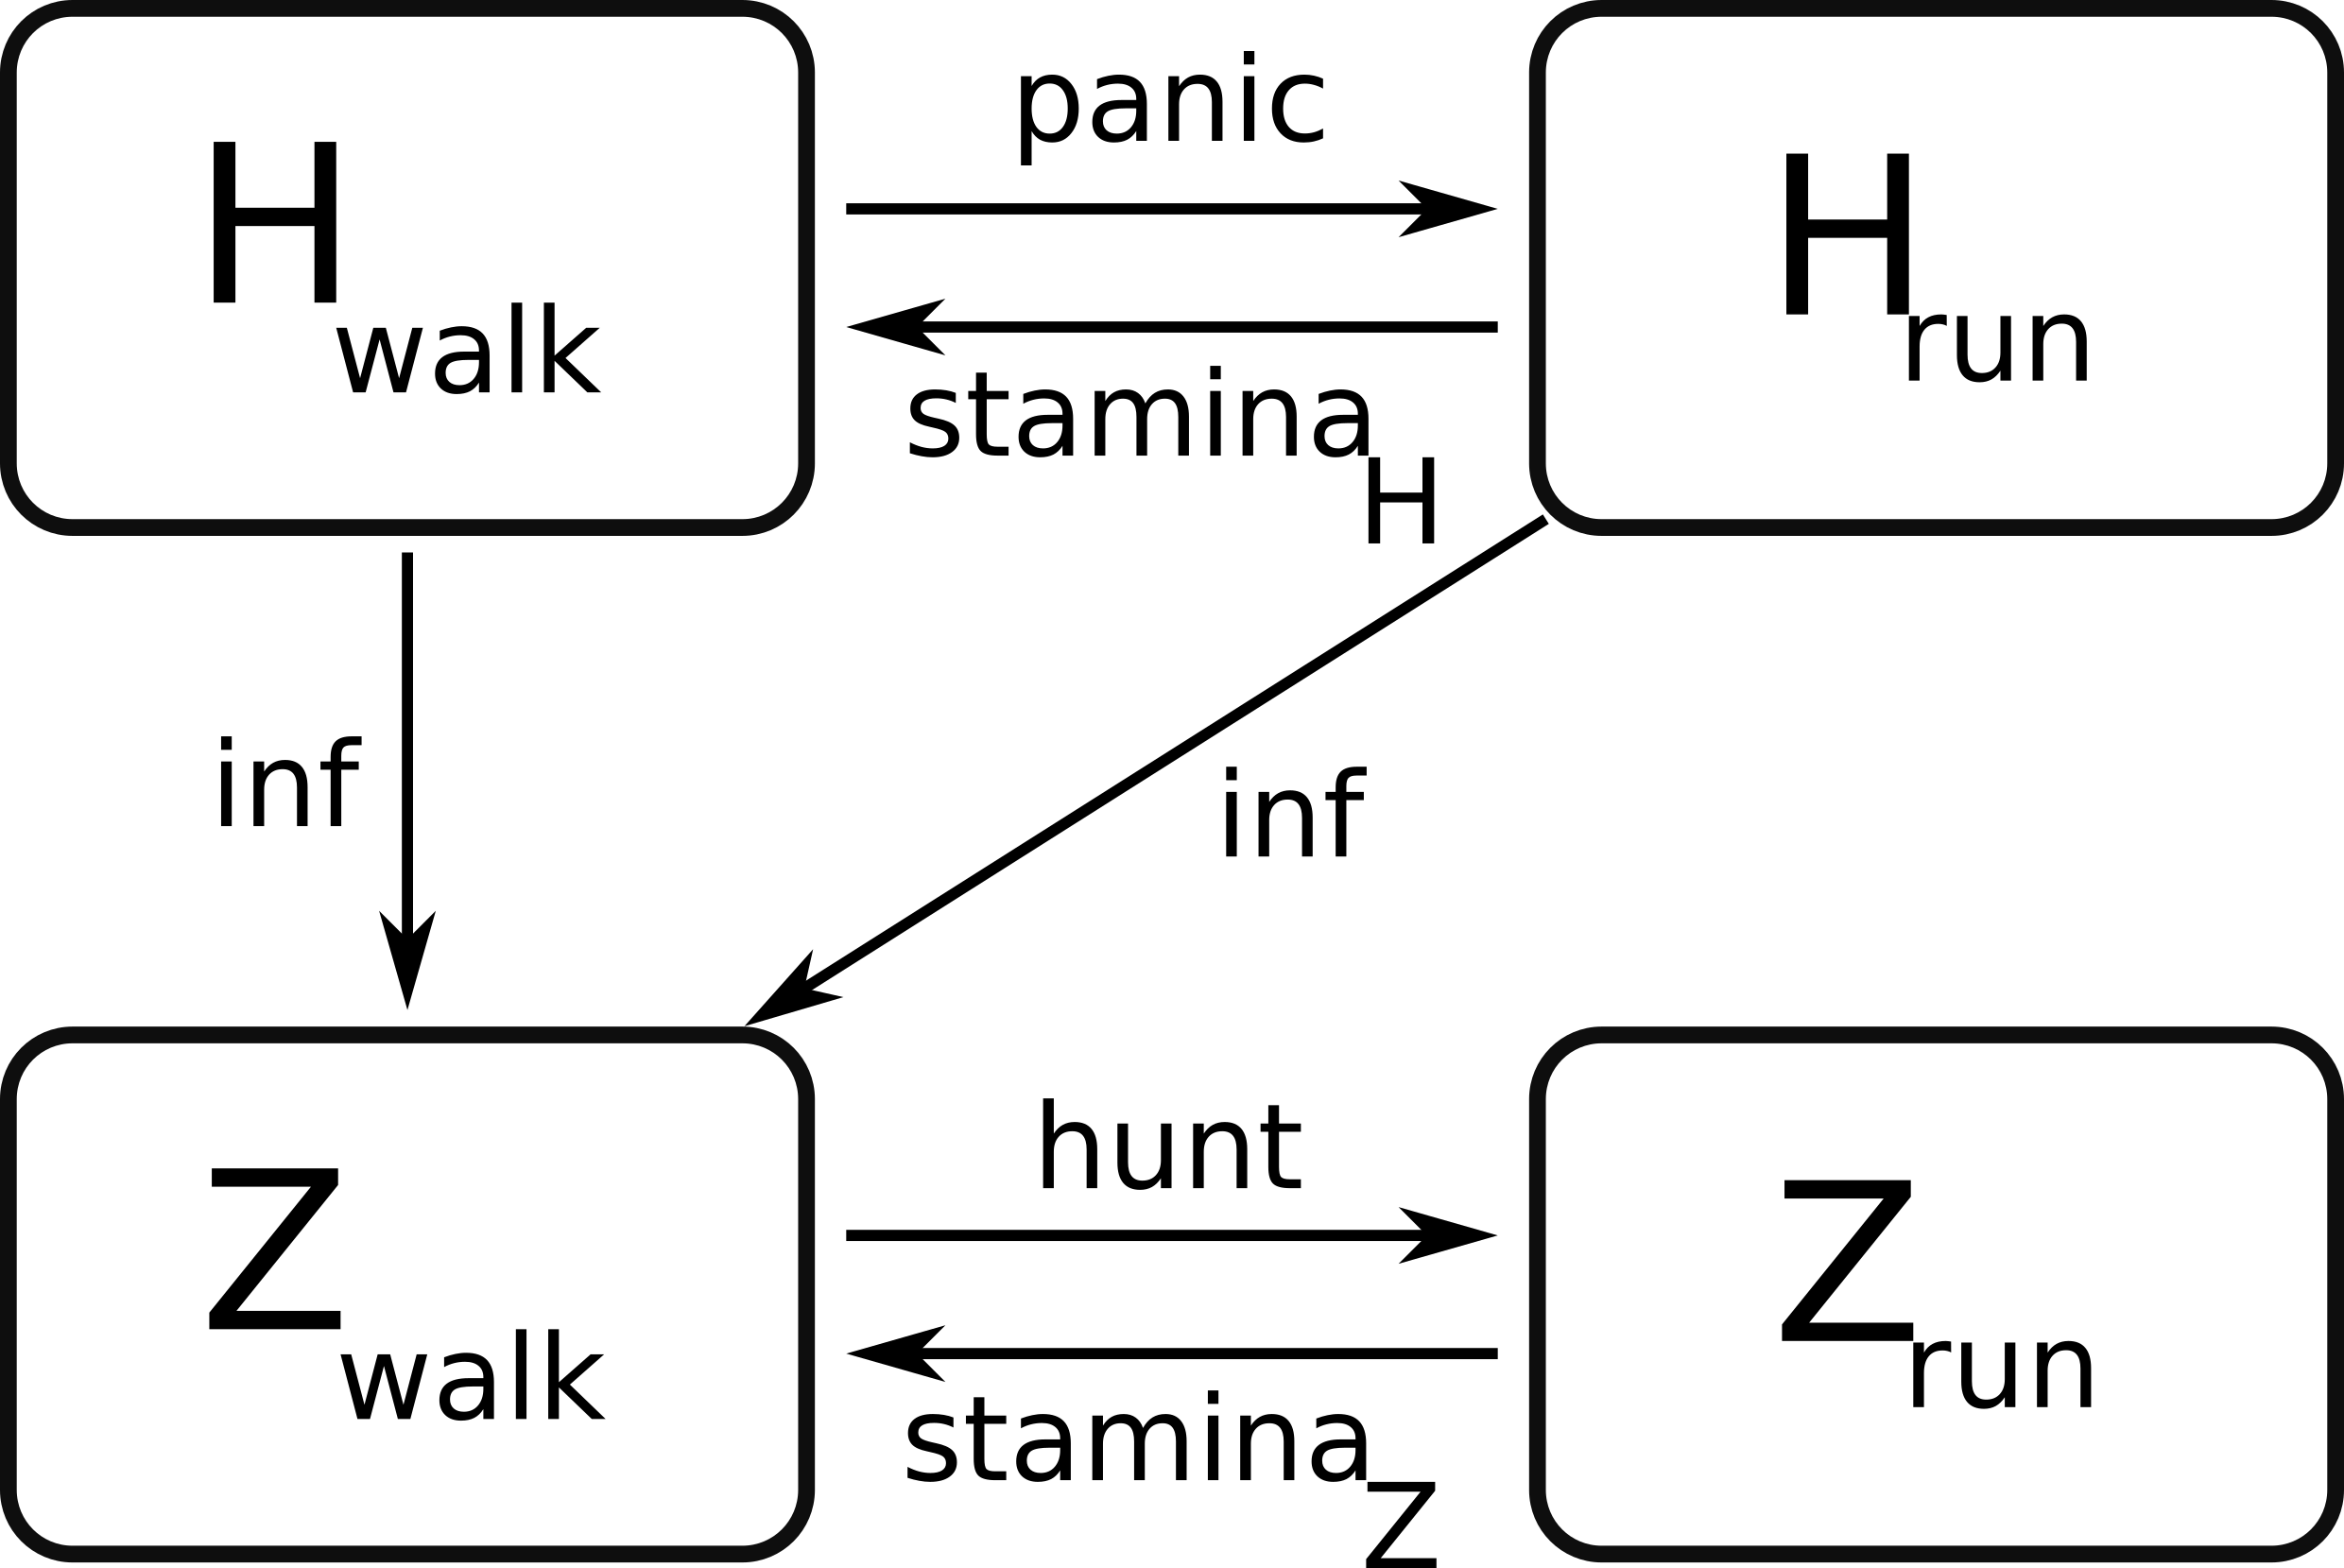
\includegraphics[width=.7\textwidth]{figures/simpleODE.png}
	\end{center}
}


\sframe{A very simple ODE model}{
	\begin{center}
	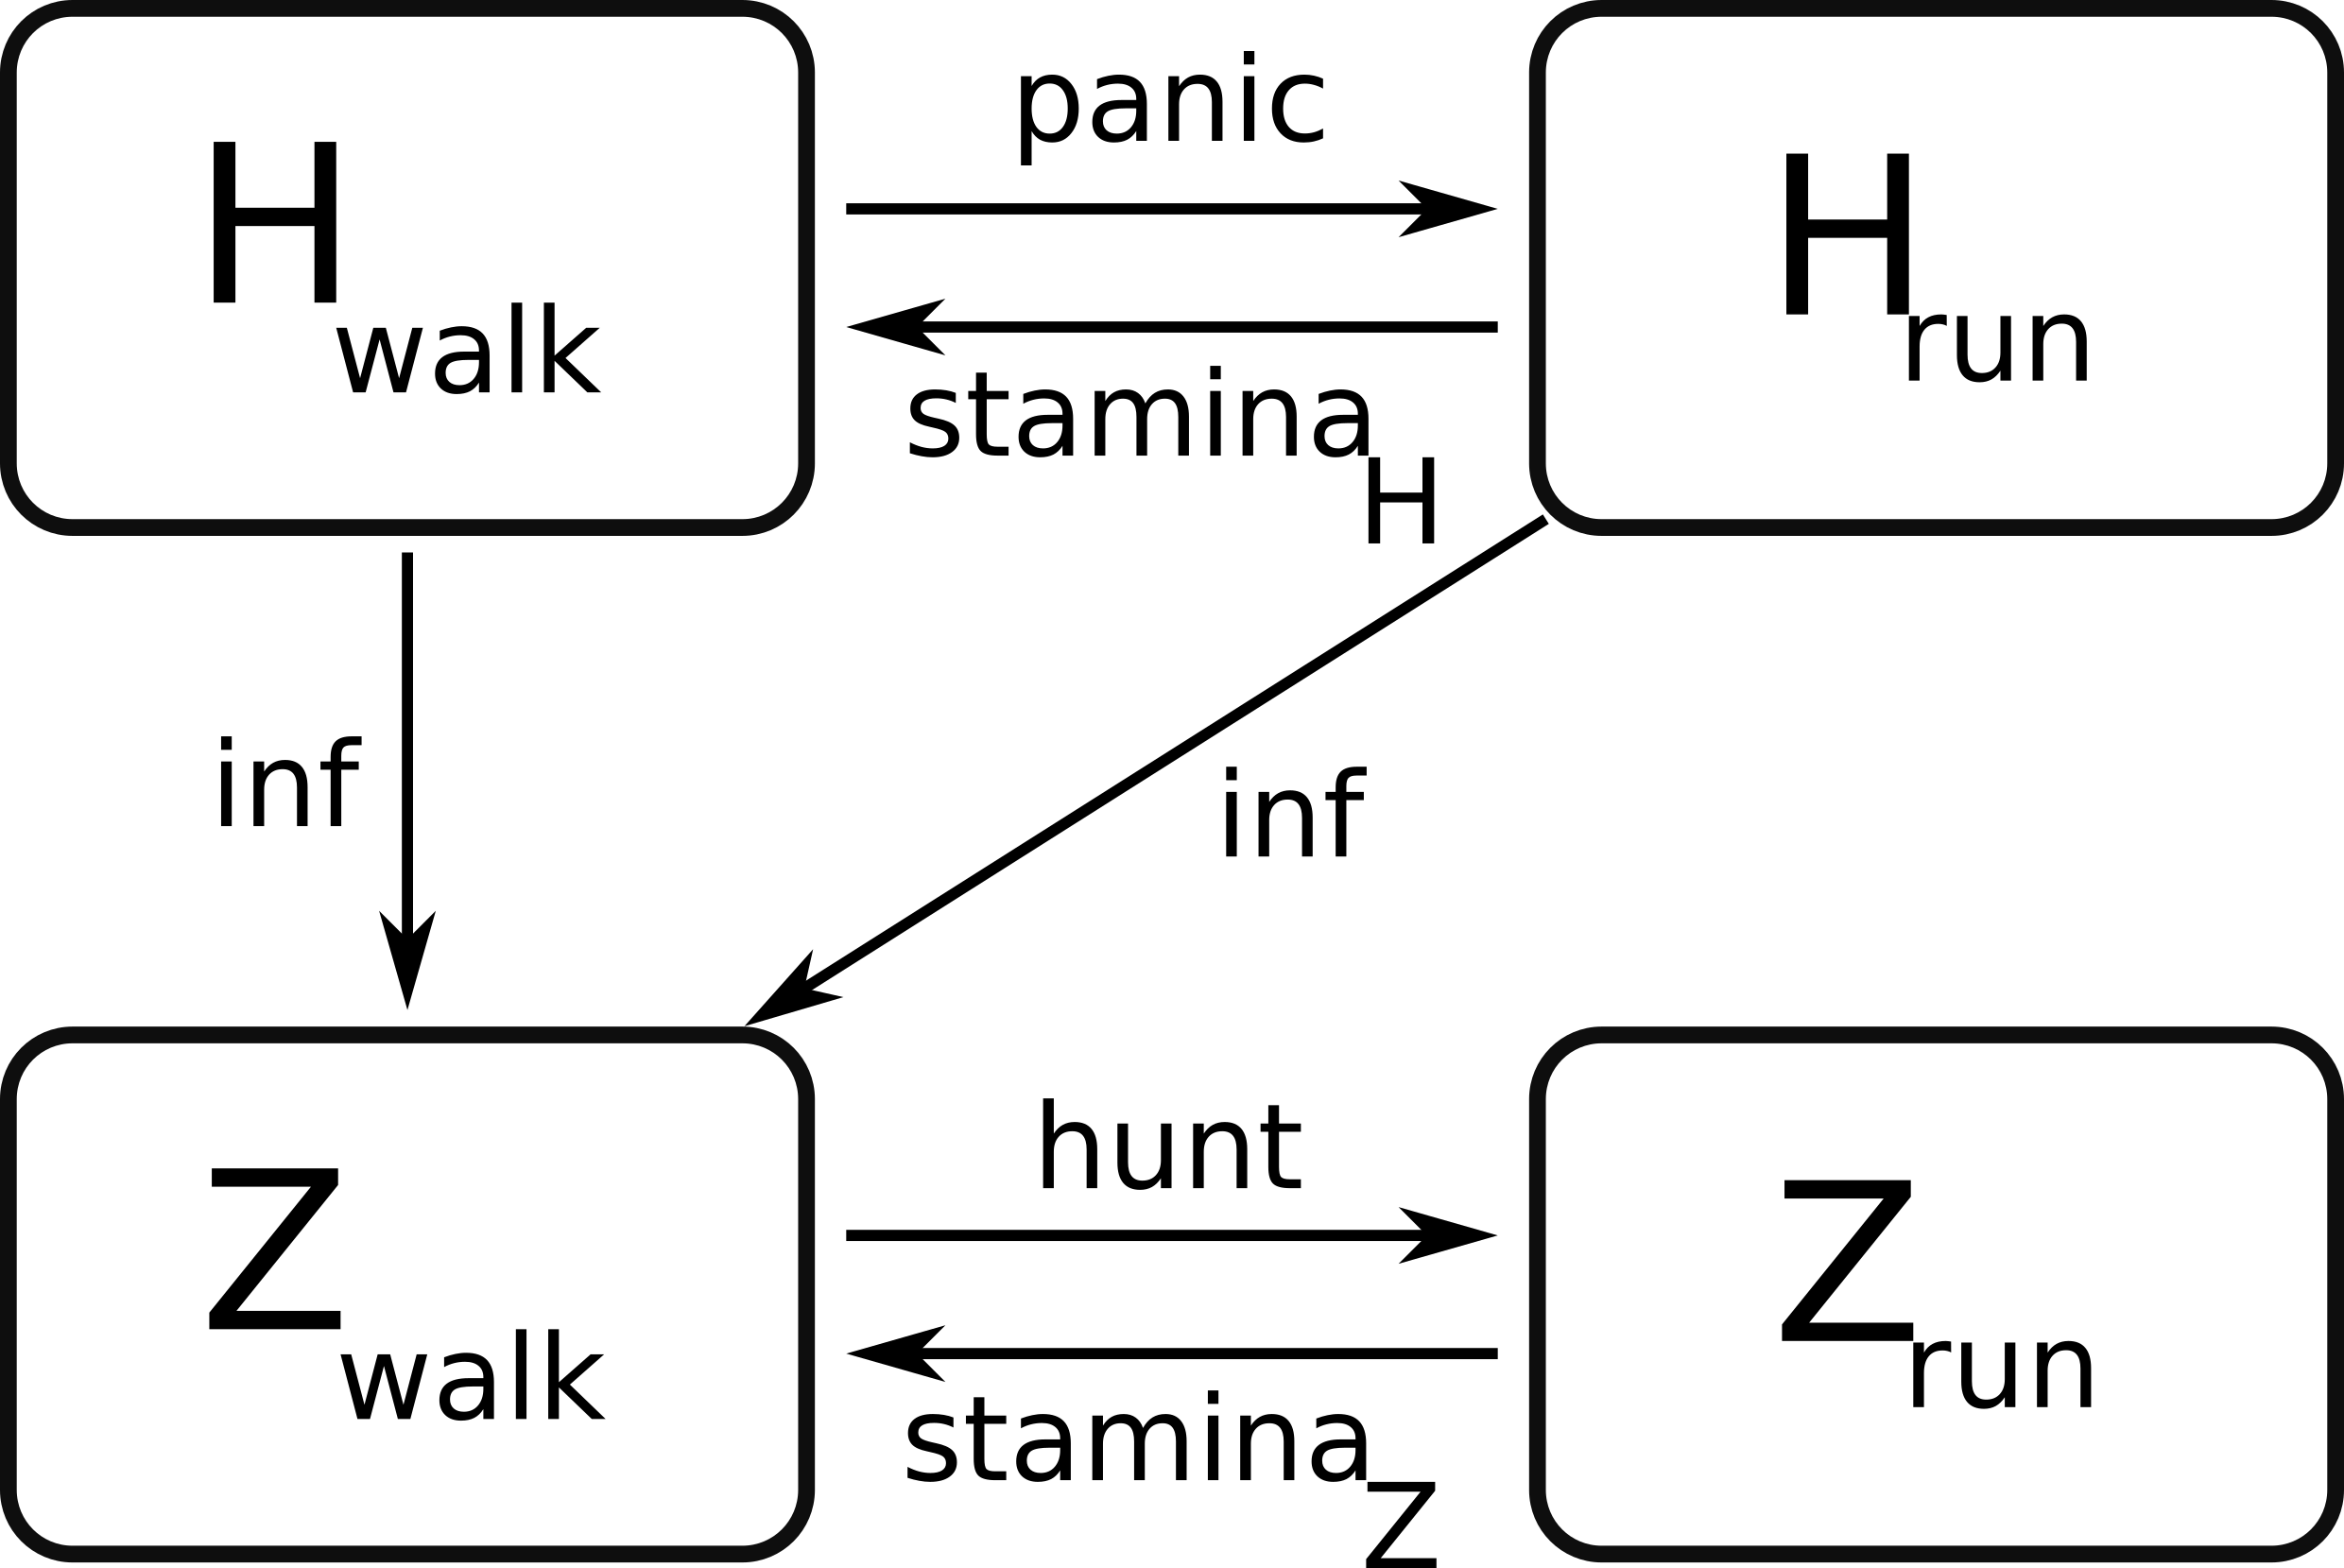
\includegraphics[width=.35\textwidth]{figures/simpleODE.png}
	\end{center}
	
	\begin{eqnarray*}
		\left\{
		\begin{array}{lcl}
			\dv{H_{walk}}{t}  & = &  -(panic + inf) * H_{walk} + exhaustH * H_{run} \\
			\tmspace{1mu}&& \\
			\dv{H_{run}}{t} & = & panic * H_{walk} - (exhaustH + inf) * H_{run} \\
			\tmspace{1mu}&& \\
			\dv{Z_{walk}}{t} & = & inf * (H_{walk} + H_{run}) - hunt * Z_{walk} + exhaustZ * Z_{run} \\
			\tmspace{1mu}&& \\
			\dv{Z_{run}}{t} & = & hunt * Z_{walk} - exhaustZ * Z_{run}
		\end{array}
		\right.
	\end{eqnarray*}
}

\sframe{A very simple ODE model}{
	\begin{eqnarray*}
		\left\{
		\begin{array}{lcl}
			N & = & H_{walk} + H_{run} + Z_{walk} + Z_{run} \\
			\tmspace{1mu}&& \\
			panic  & = &  panic_0 * (Z_{walk} + Z_{run}) / N \\
			\tmspace{1mu}&& \\
			hunt & = & hunt0 * (H_{walk} + H_{run}) / N
		\end{array}
		\right.
	\end{eqnarray*}
}


\section{Exploration}

\sframe{First step: Calibrate}{
	\begin{center}
	We have some real time series of zombie invasion \\
	$\rightarrow$ find the parameter values to best fit them
	\end{center}
	
	\bigskip
	
	\visible<2>{
	\begin{center}
	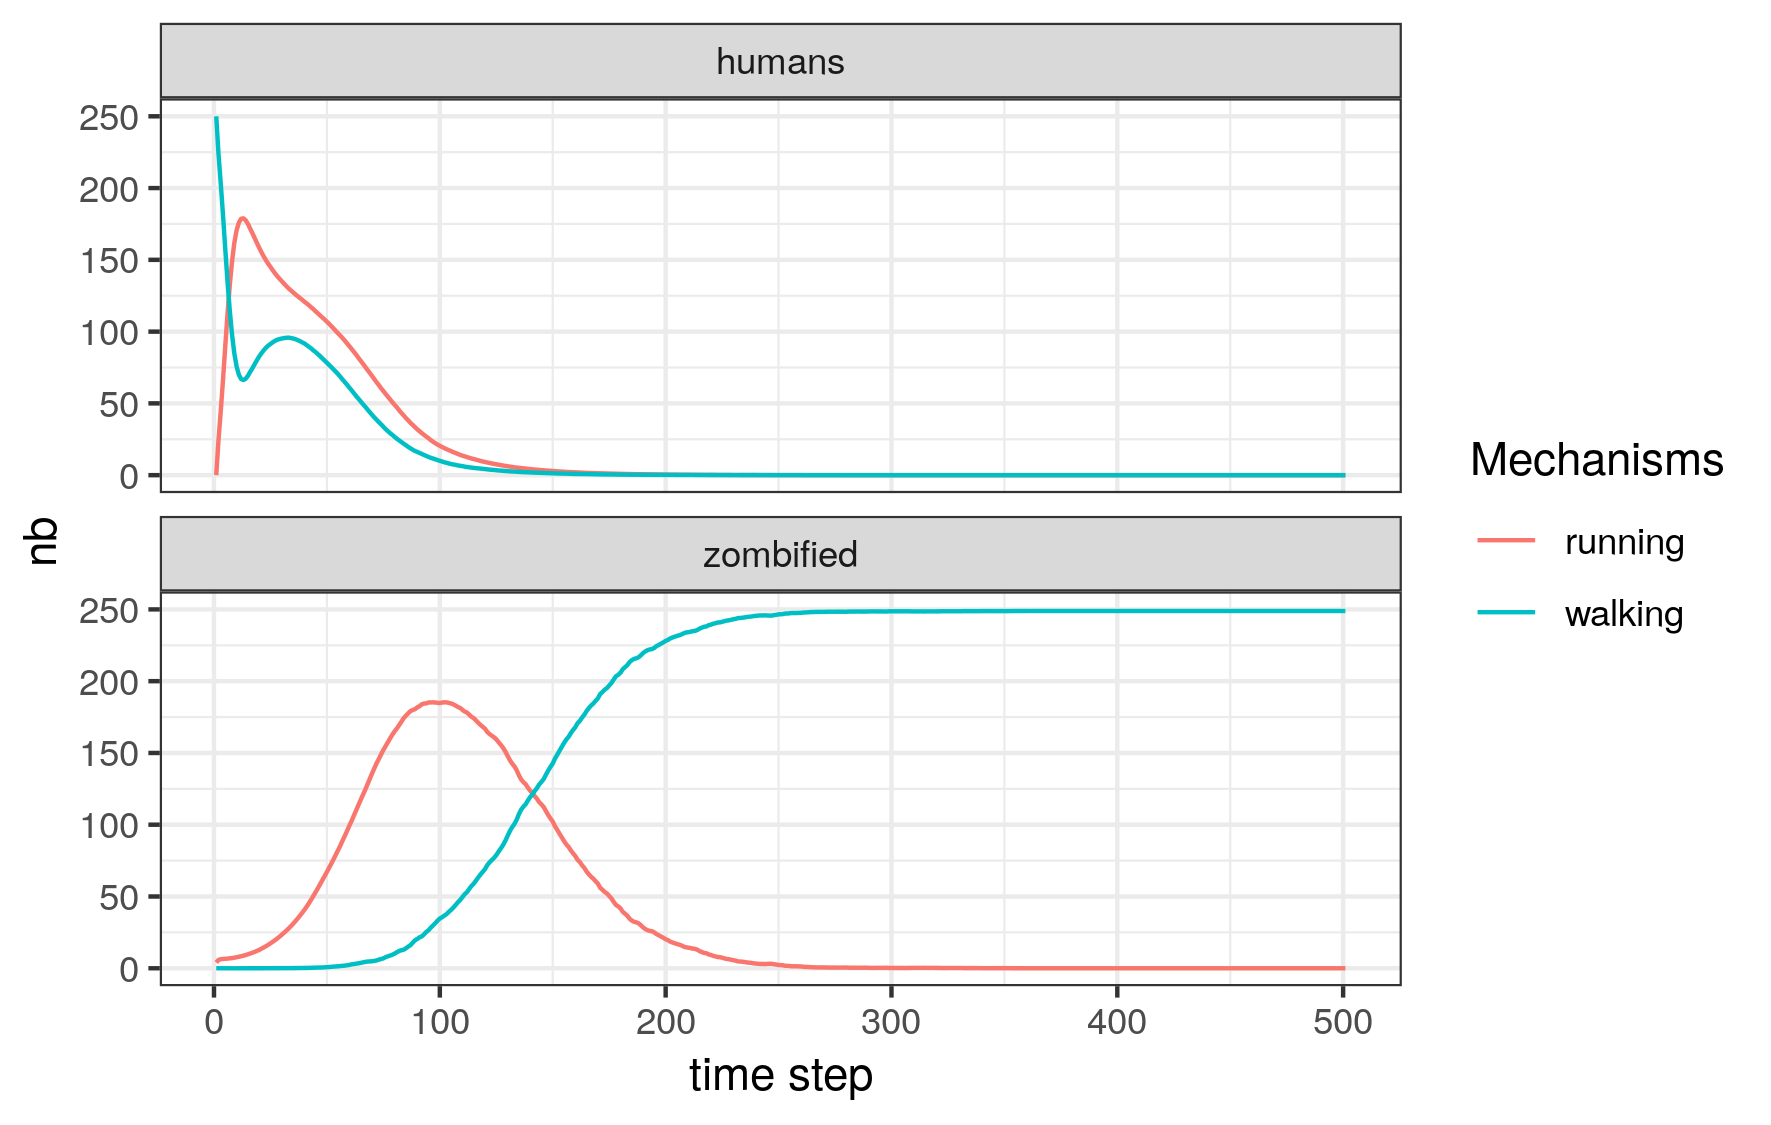
\includegraphics[width=.9\textwidth]{figures/ABMdynamics.png}
	\end{center}
	}
}
	
\sframe{First step: Calibrate}{
	\head{Process}
	
	\begin{itemize}
		\visible<2->{\item Embed the model in OpenMOLE}
		\visible<3->{\item Define a fitness function}
		\visible<4->{\item Write a calibration task}
	\end{itemize}
}


\sframe{Calibration results}{
\begin{columns}
\begin{column}{.3\textwidth}
	\head{Parameter set}
	\begin{table}
	\begin{center}
	\makegapedcells
	\begin{tabular}{ll}
		\head{$panic_0$} & 7.25\\
		\head{$stamina_H$} & 0.99\\
		\head{$hunt_0$} & 10.15\\
		\head{$stamina_Z$} & 1.28\\
		\head{$inf$} & 0.02\\
		{\color{primaryGreenOM}fitness} & 780~394
	\end{tabular}
	\end{center}
	\end{table}
\end{column}

\begin{column}{.8\textwidth}
	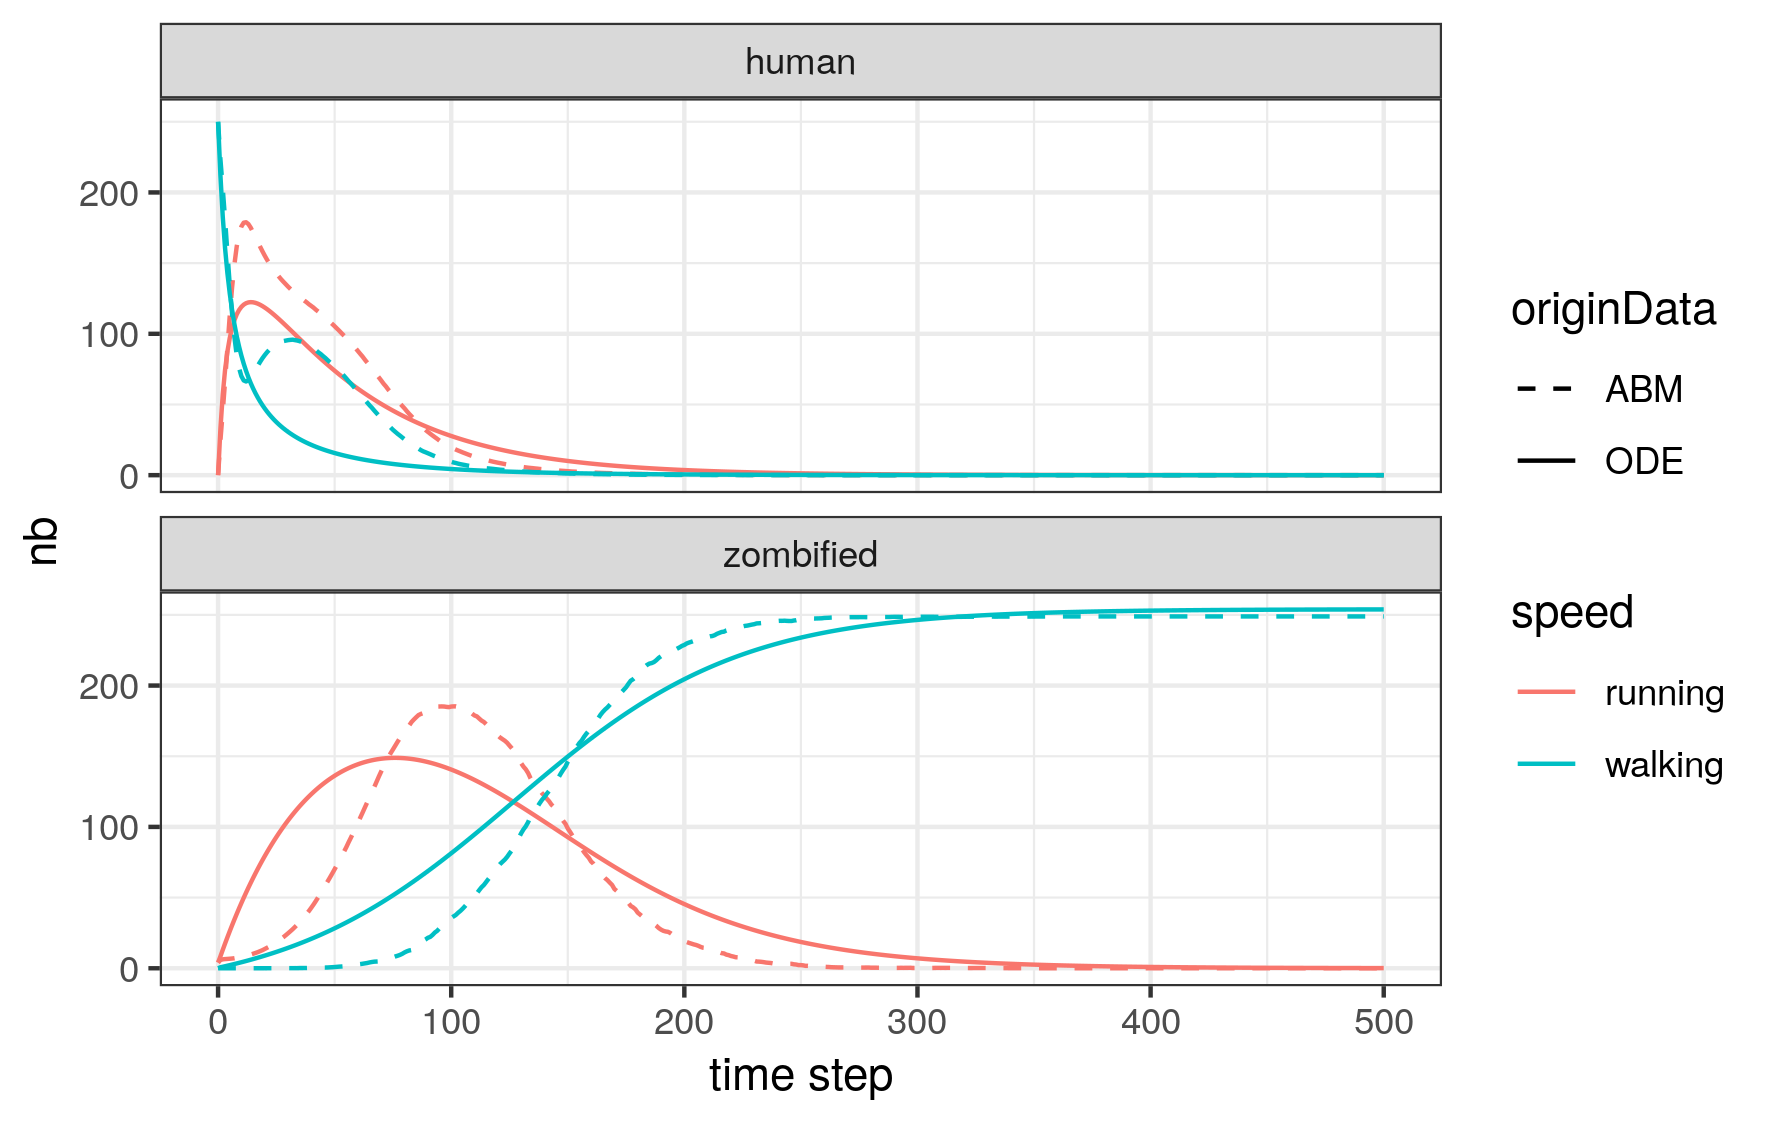
\includegraphics[width=\textwidth]{figures/calib_dynamics.png}
\end{column}
\end{columns}
}


\sframe{Second step: Profiles}{
	Profiles for each of the 5 parameters:\\
	$rightarrow$ $panic_0$, $stamina_H$, $hunt_0$, $stamina_Z$, $inf_0$
}


\sframe{Profiles}{
	\begin{center}
	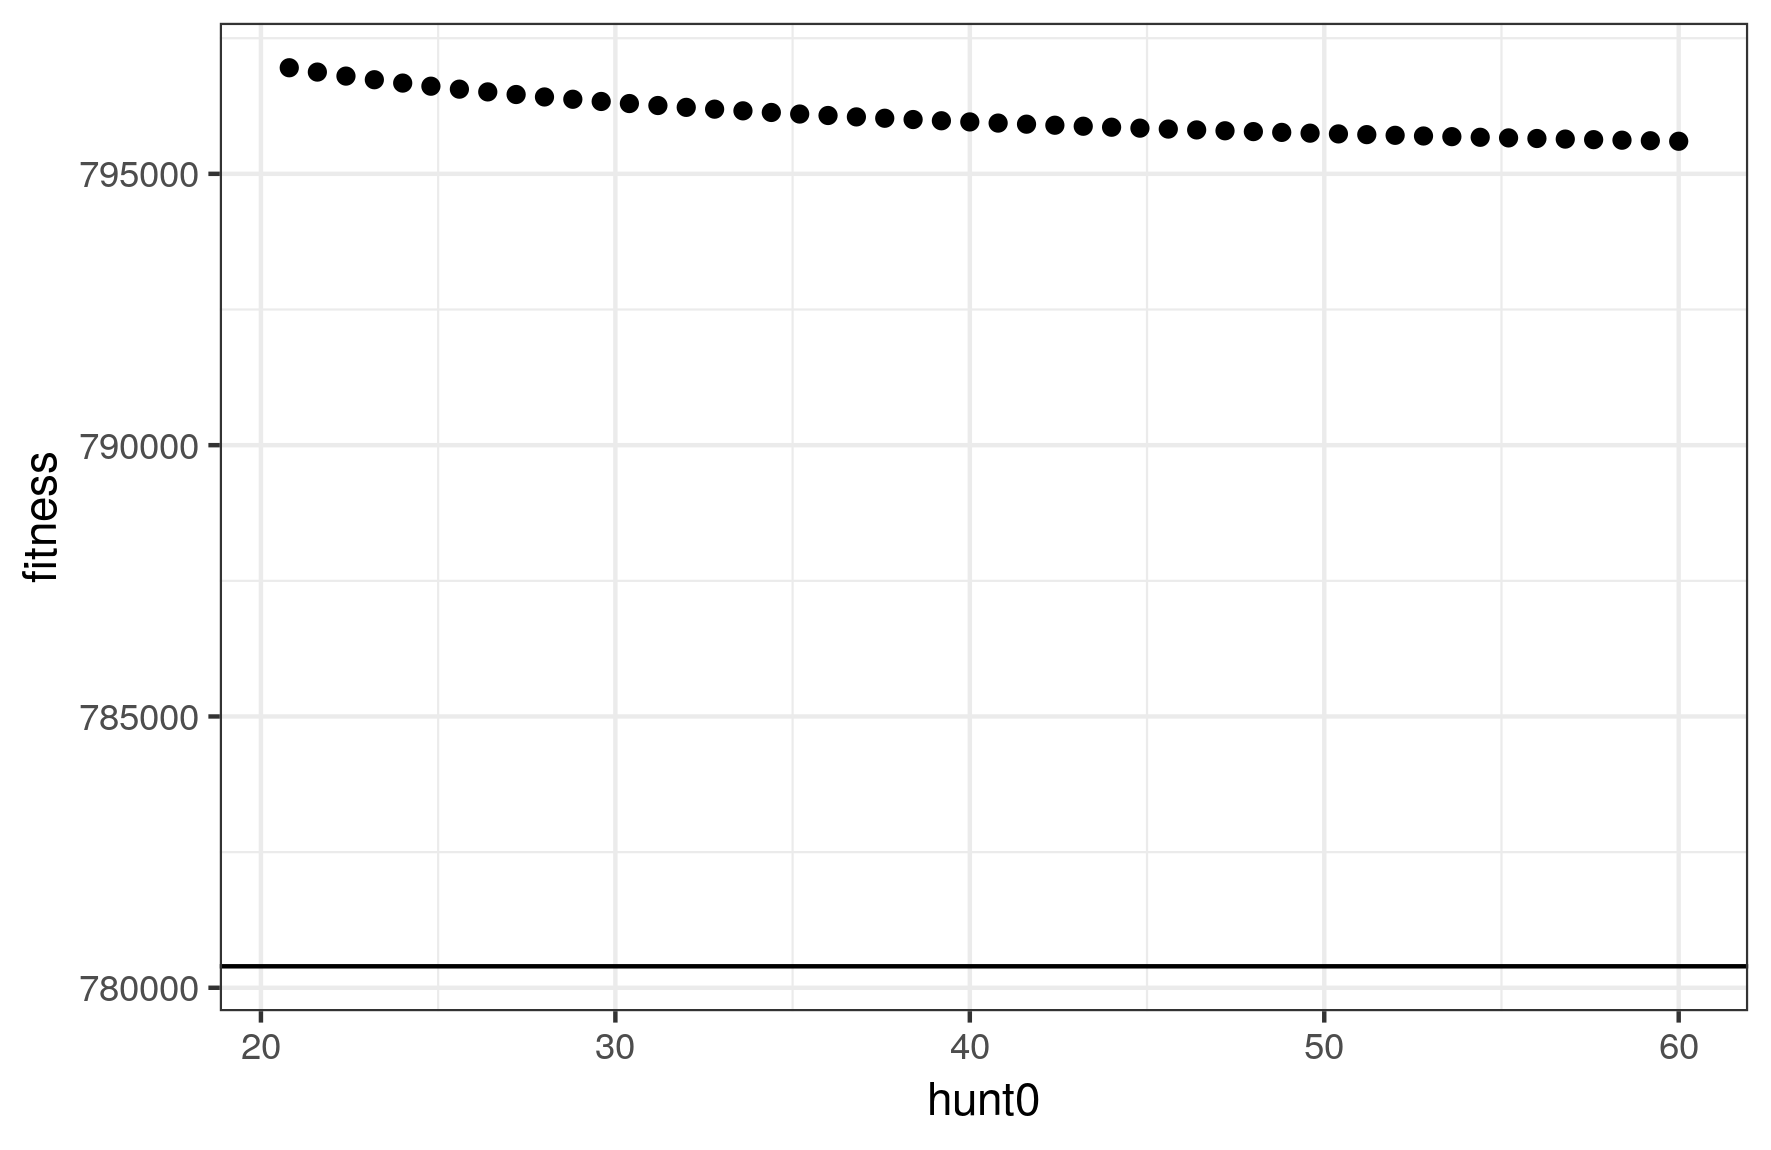
\includegraphics[width=\textwidth]{figures/profile_hunt0.png}
	\end{center}
}


\sframe{Profiles}{
	\begin{center}
	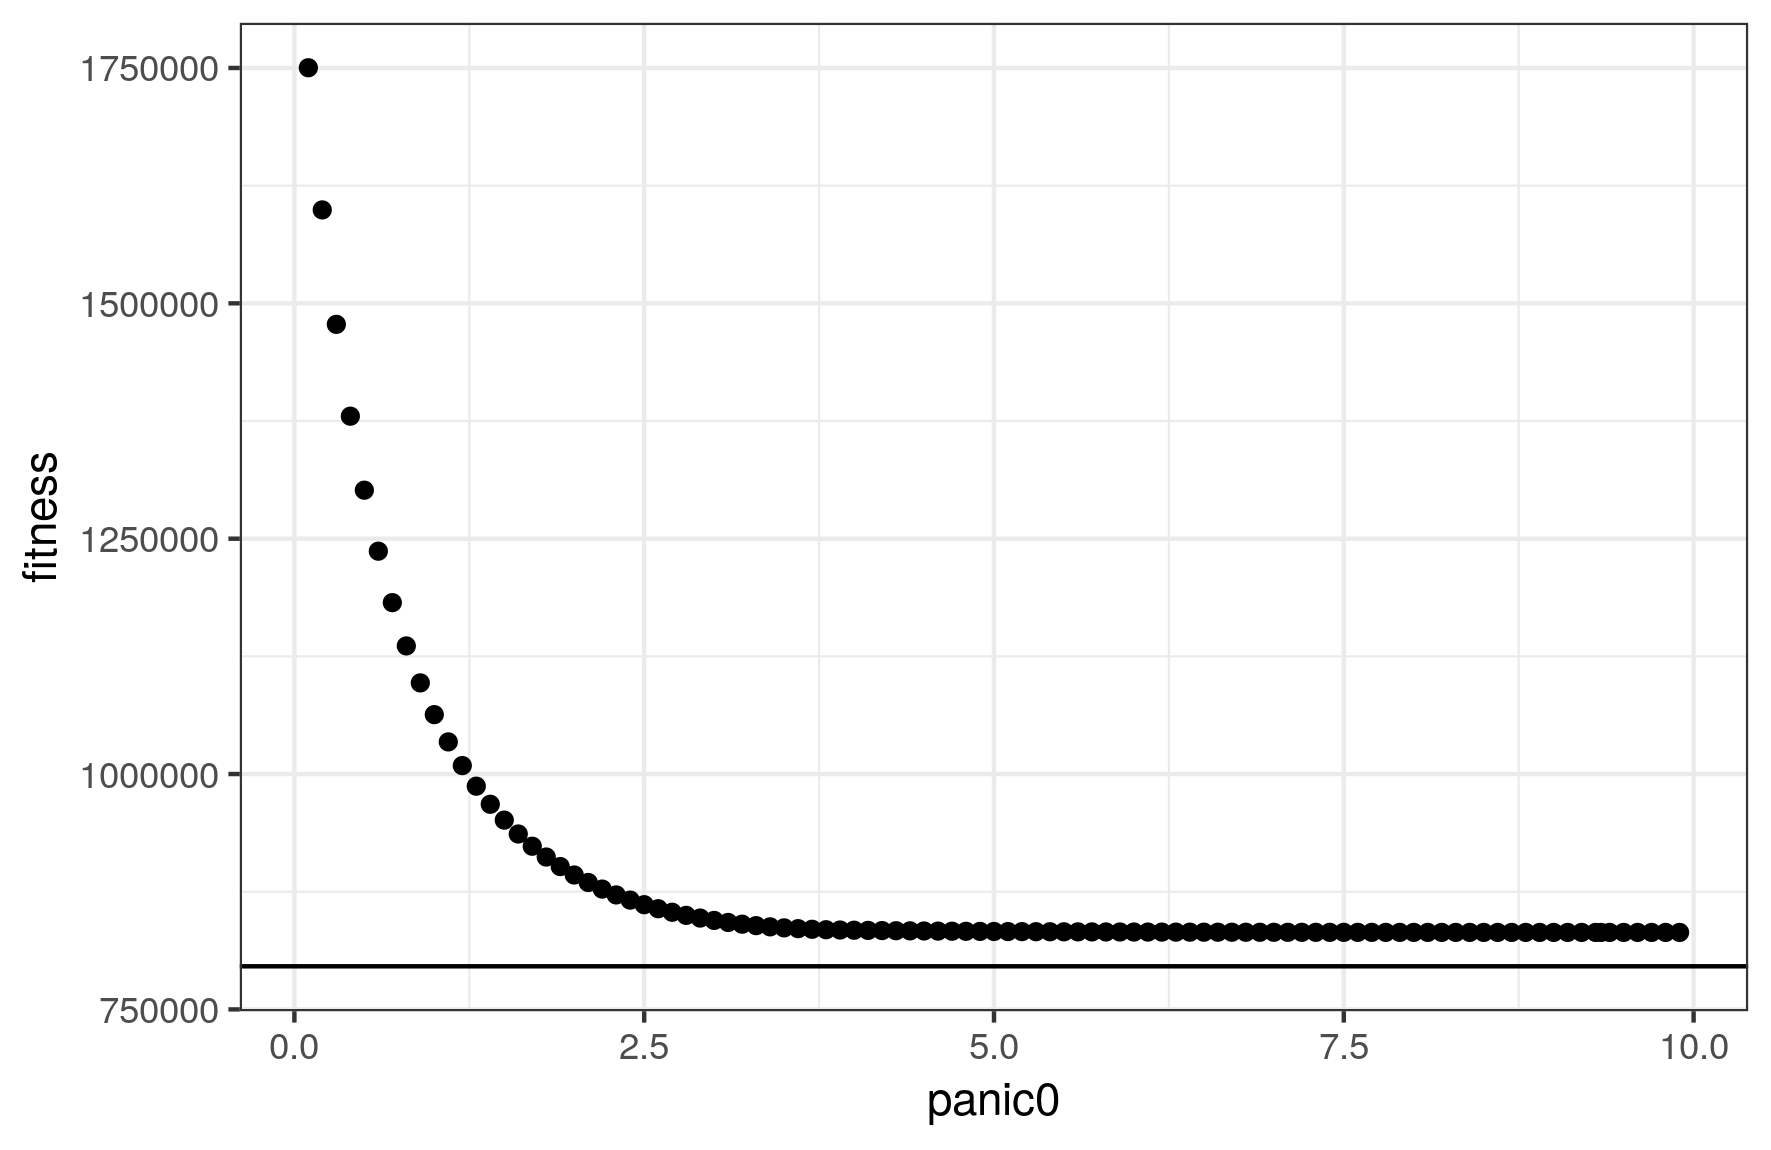
\includegraphics[width=\textwidth]{figures/profile_panic0.png}
	\end{center}
}


\sframe{Profiles}{
	\begin{center}
	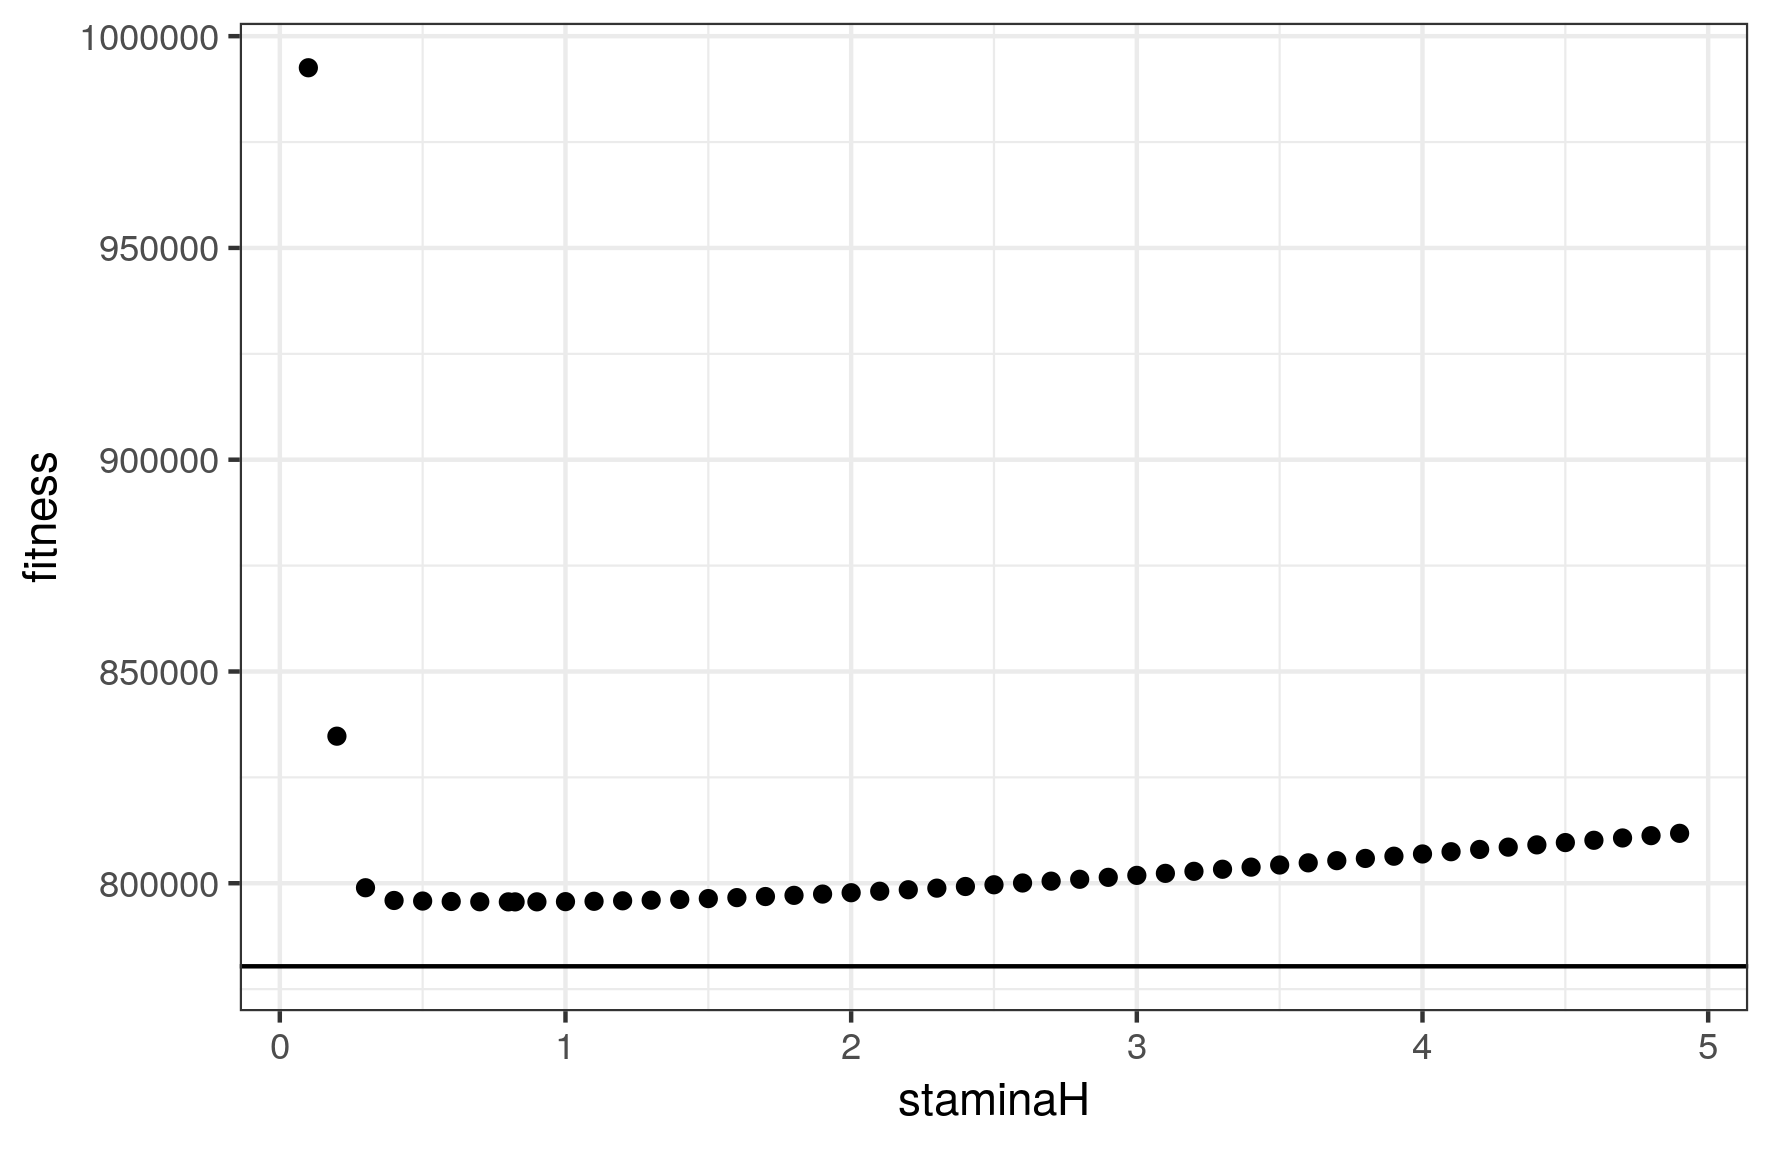
\includegraphics[width=\textwidth]{figures/profile_staminaH.png}
	\end{center}
}


\sframe{Profiles}{
	\begin{center}
	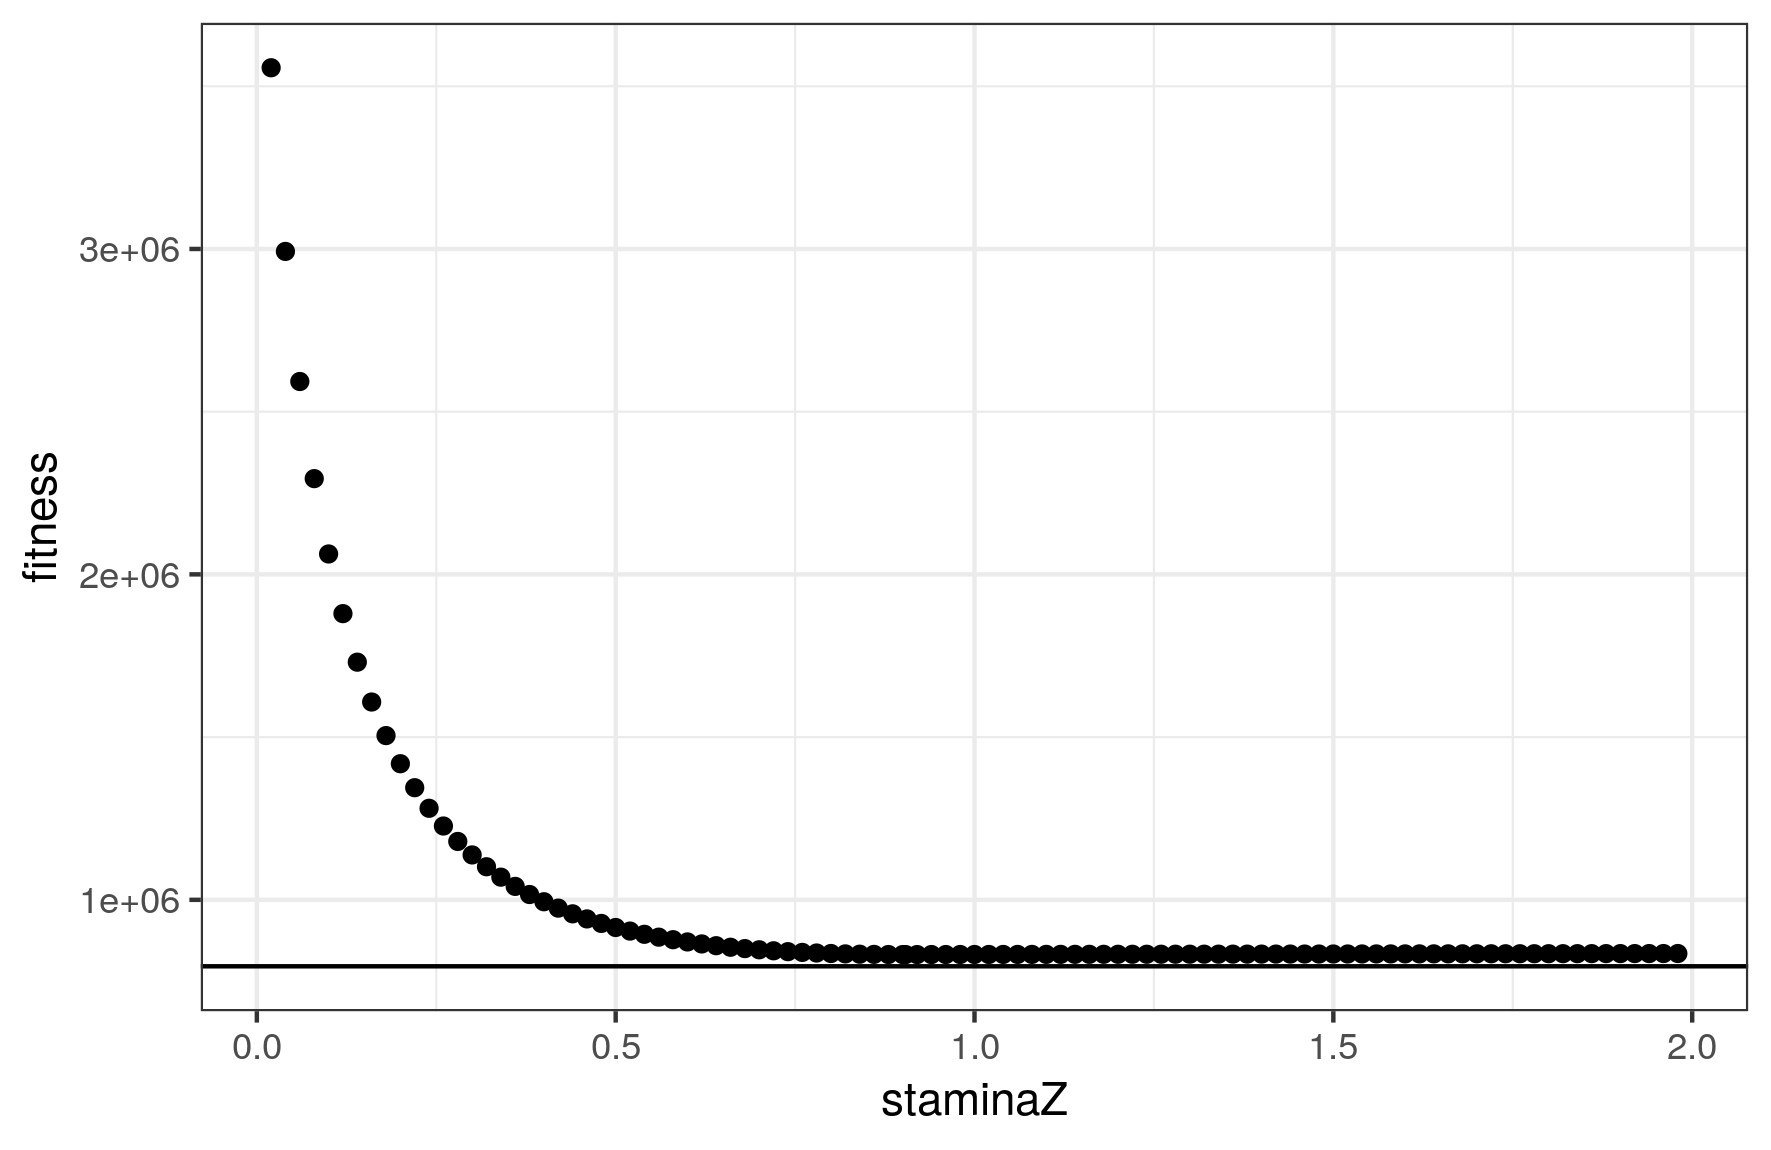
\includegraphics[width=\textwidth]{figures/profile_staminaZ.png}
	\end{center}
}


\sframe{Profiles}{
	\begin{center}
	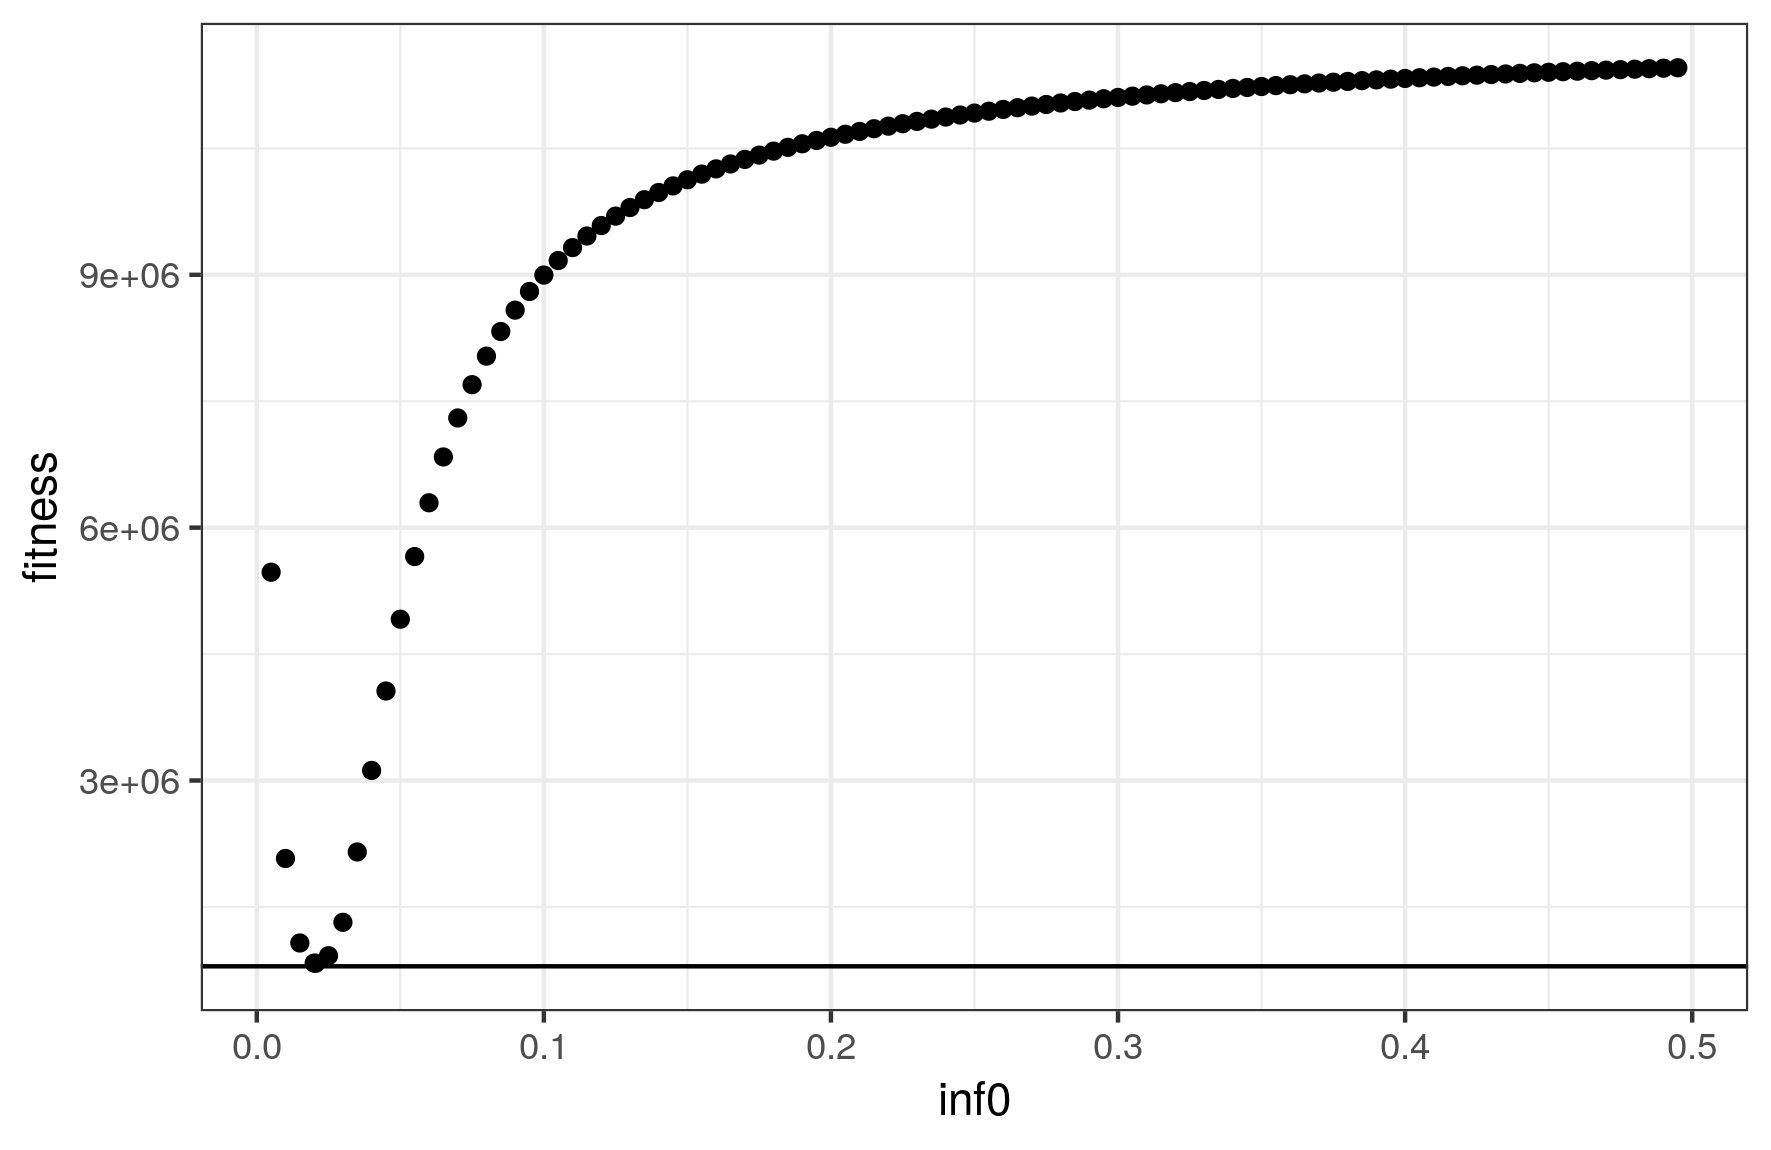
\includegraphics[width=\textwidth]{figures/profile_inf0.png}
	\end{center}
}


\section{Adding complexity}

\sframe{New mechanisms}{
	\begin{center}
	What mechanisms could we add to better represent the complexity of our Zombie situation?
	\end{center}
	
	\bigskip
	
	\visible<2->{
	\head{The parcimony issue}
	
	\begin{itemize}
		\visible<3->{\item Do the new mechanisms really improve the fitness?}
		\visible<4->{\item Do we need them all?}
		\visible<5->{\item What are the best combinations?}
	\end{itemize}
	}
}


\sframe{Study our model's parcimony}{
	\head{Process}
	
	\begin{itemize}[<+->]
		\item Embed the model in OpenMOLE \head{DONE}
		\item Define a \head{second} fitness function
		\item \head{Modify} the calibration task
	\end{itemize}
}


\sframe{Pareto front}{
	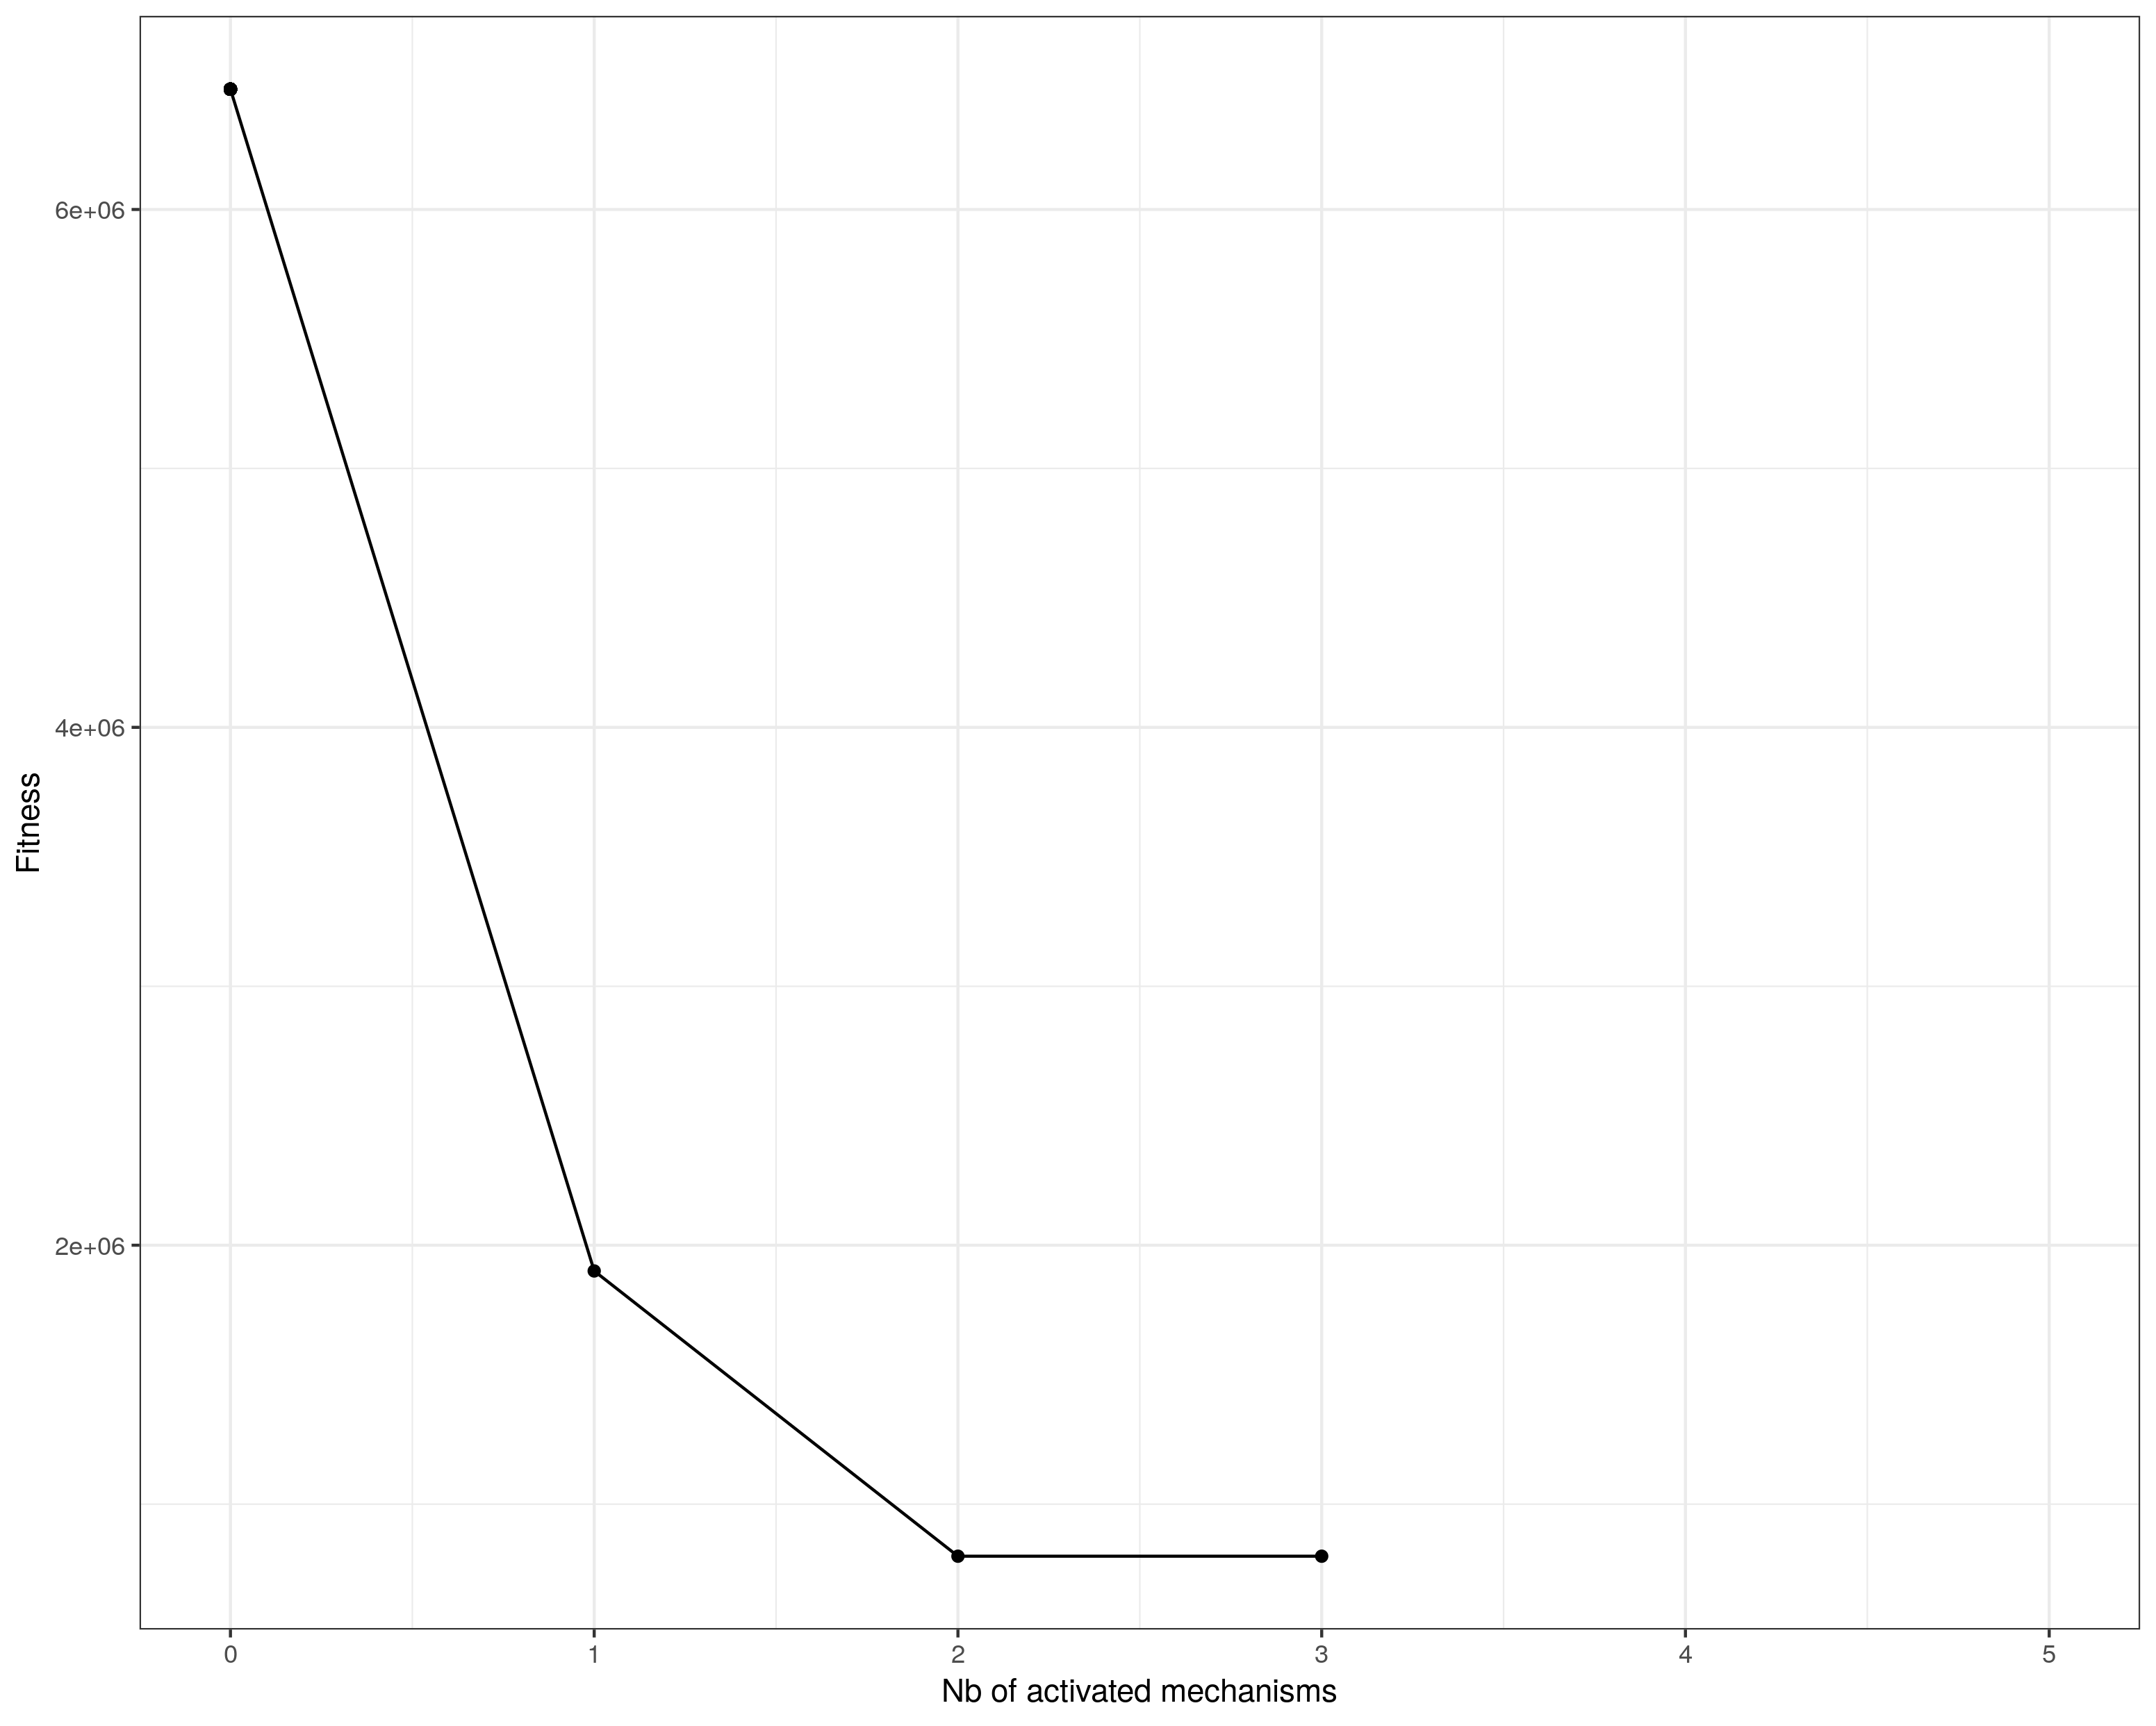
\includegraphics[width=\textwidth]{figures/parcimony/plot_parcimony.png}
}


\sframe{Dynamics for 0 mechanism activated}{
	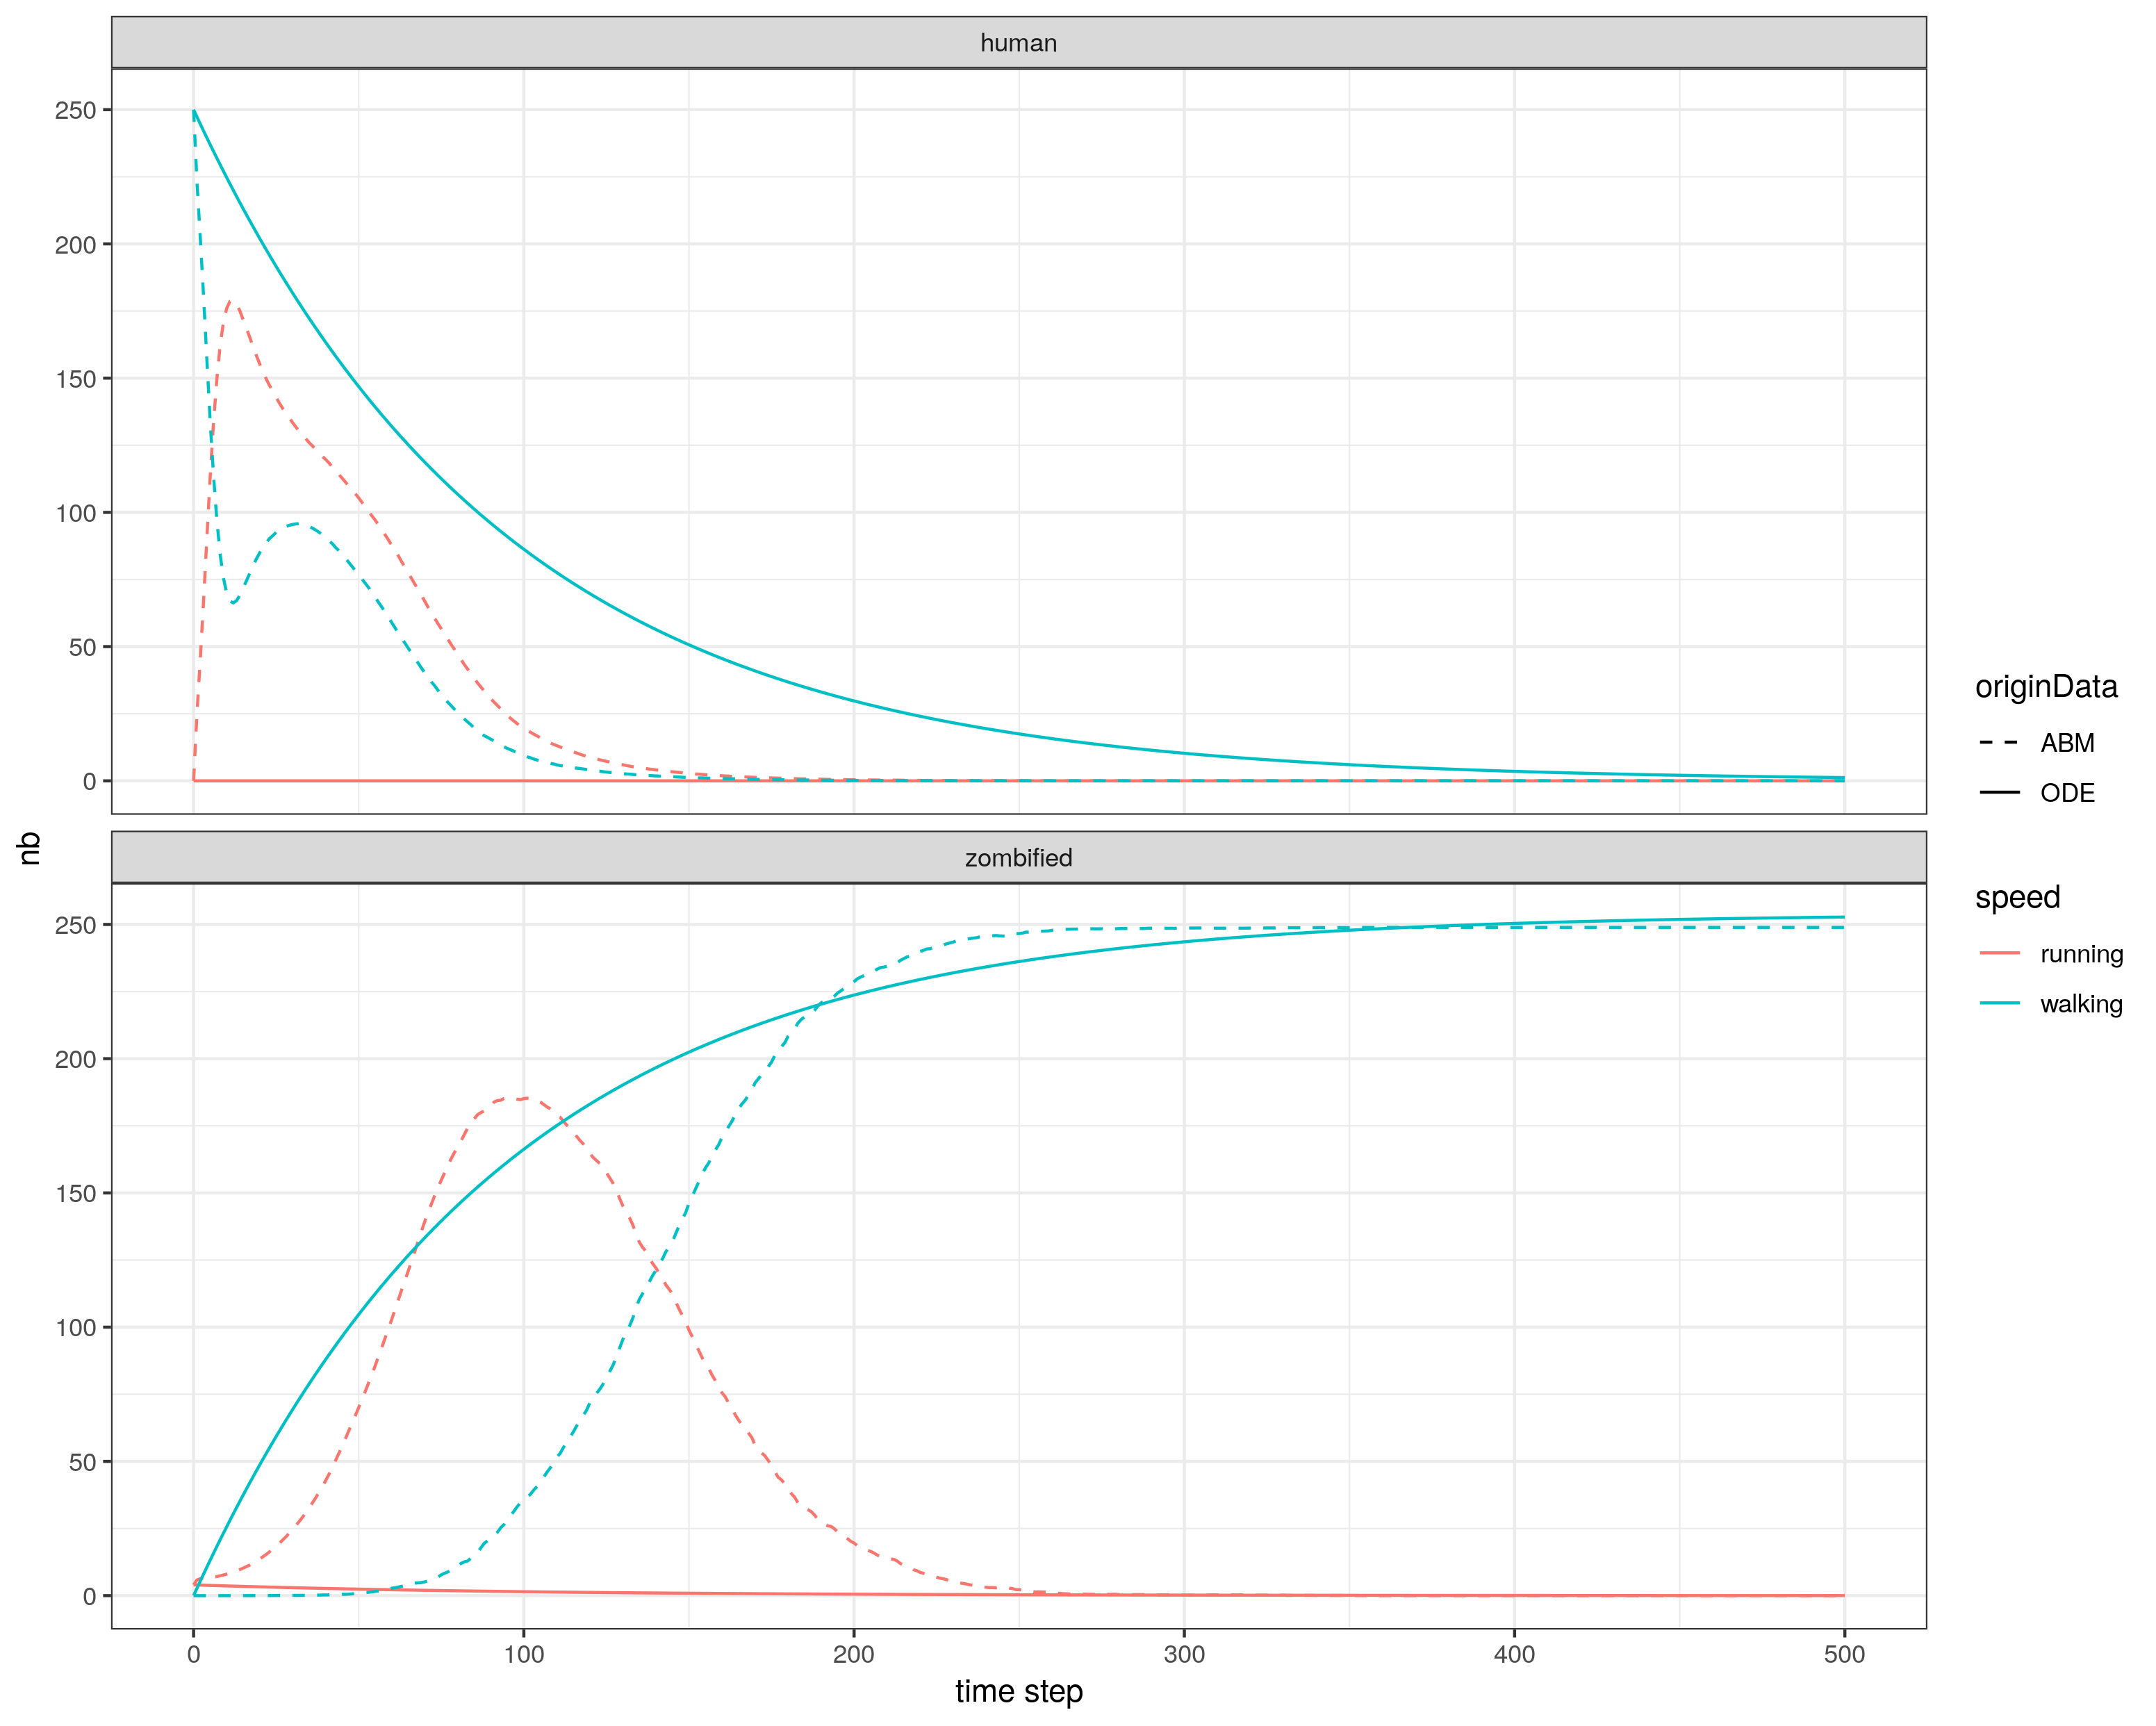
\includegraphics[width=\textwidth]{figures/parcimony/parcimony_dynamics_0.png}
}


\sframe{Dynamics for 1 mechanism activated}{
	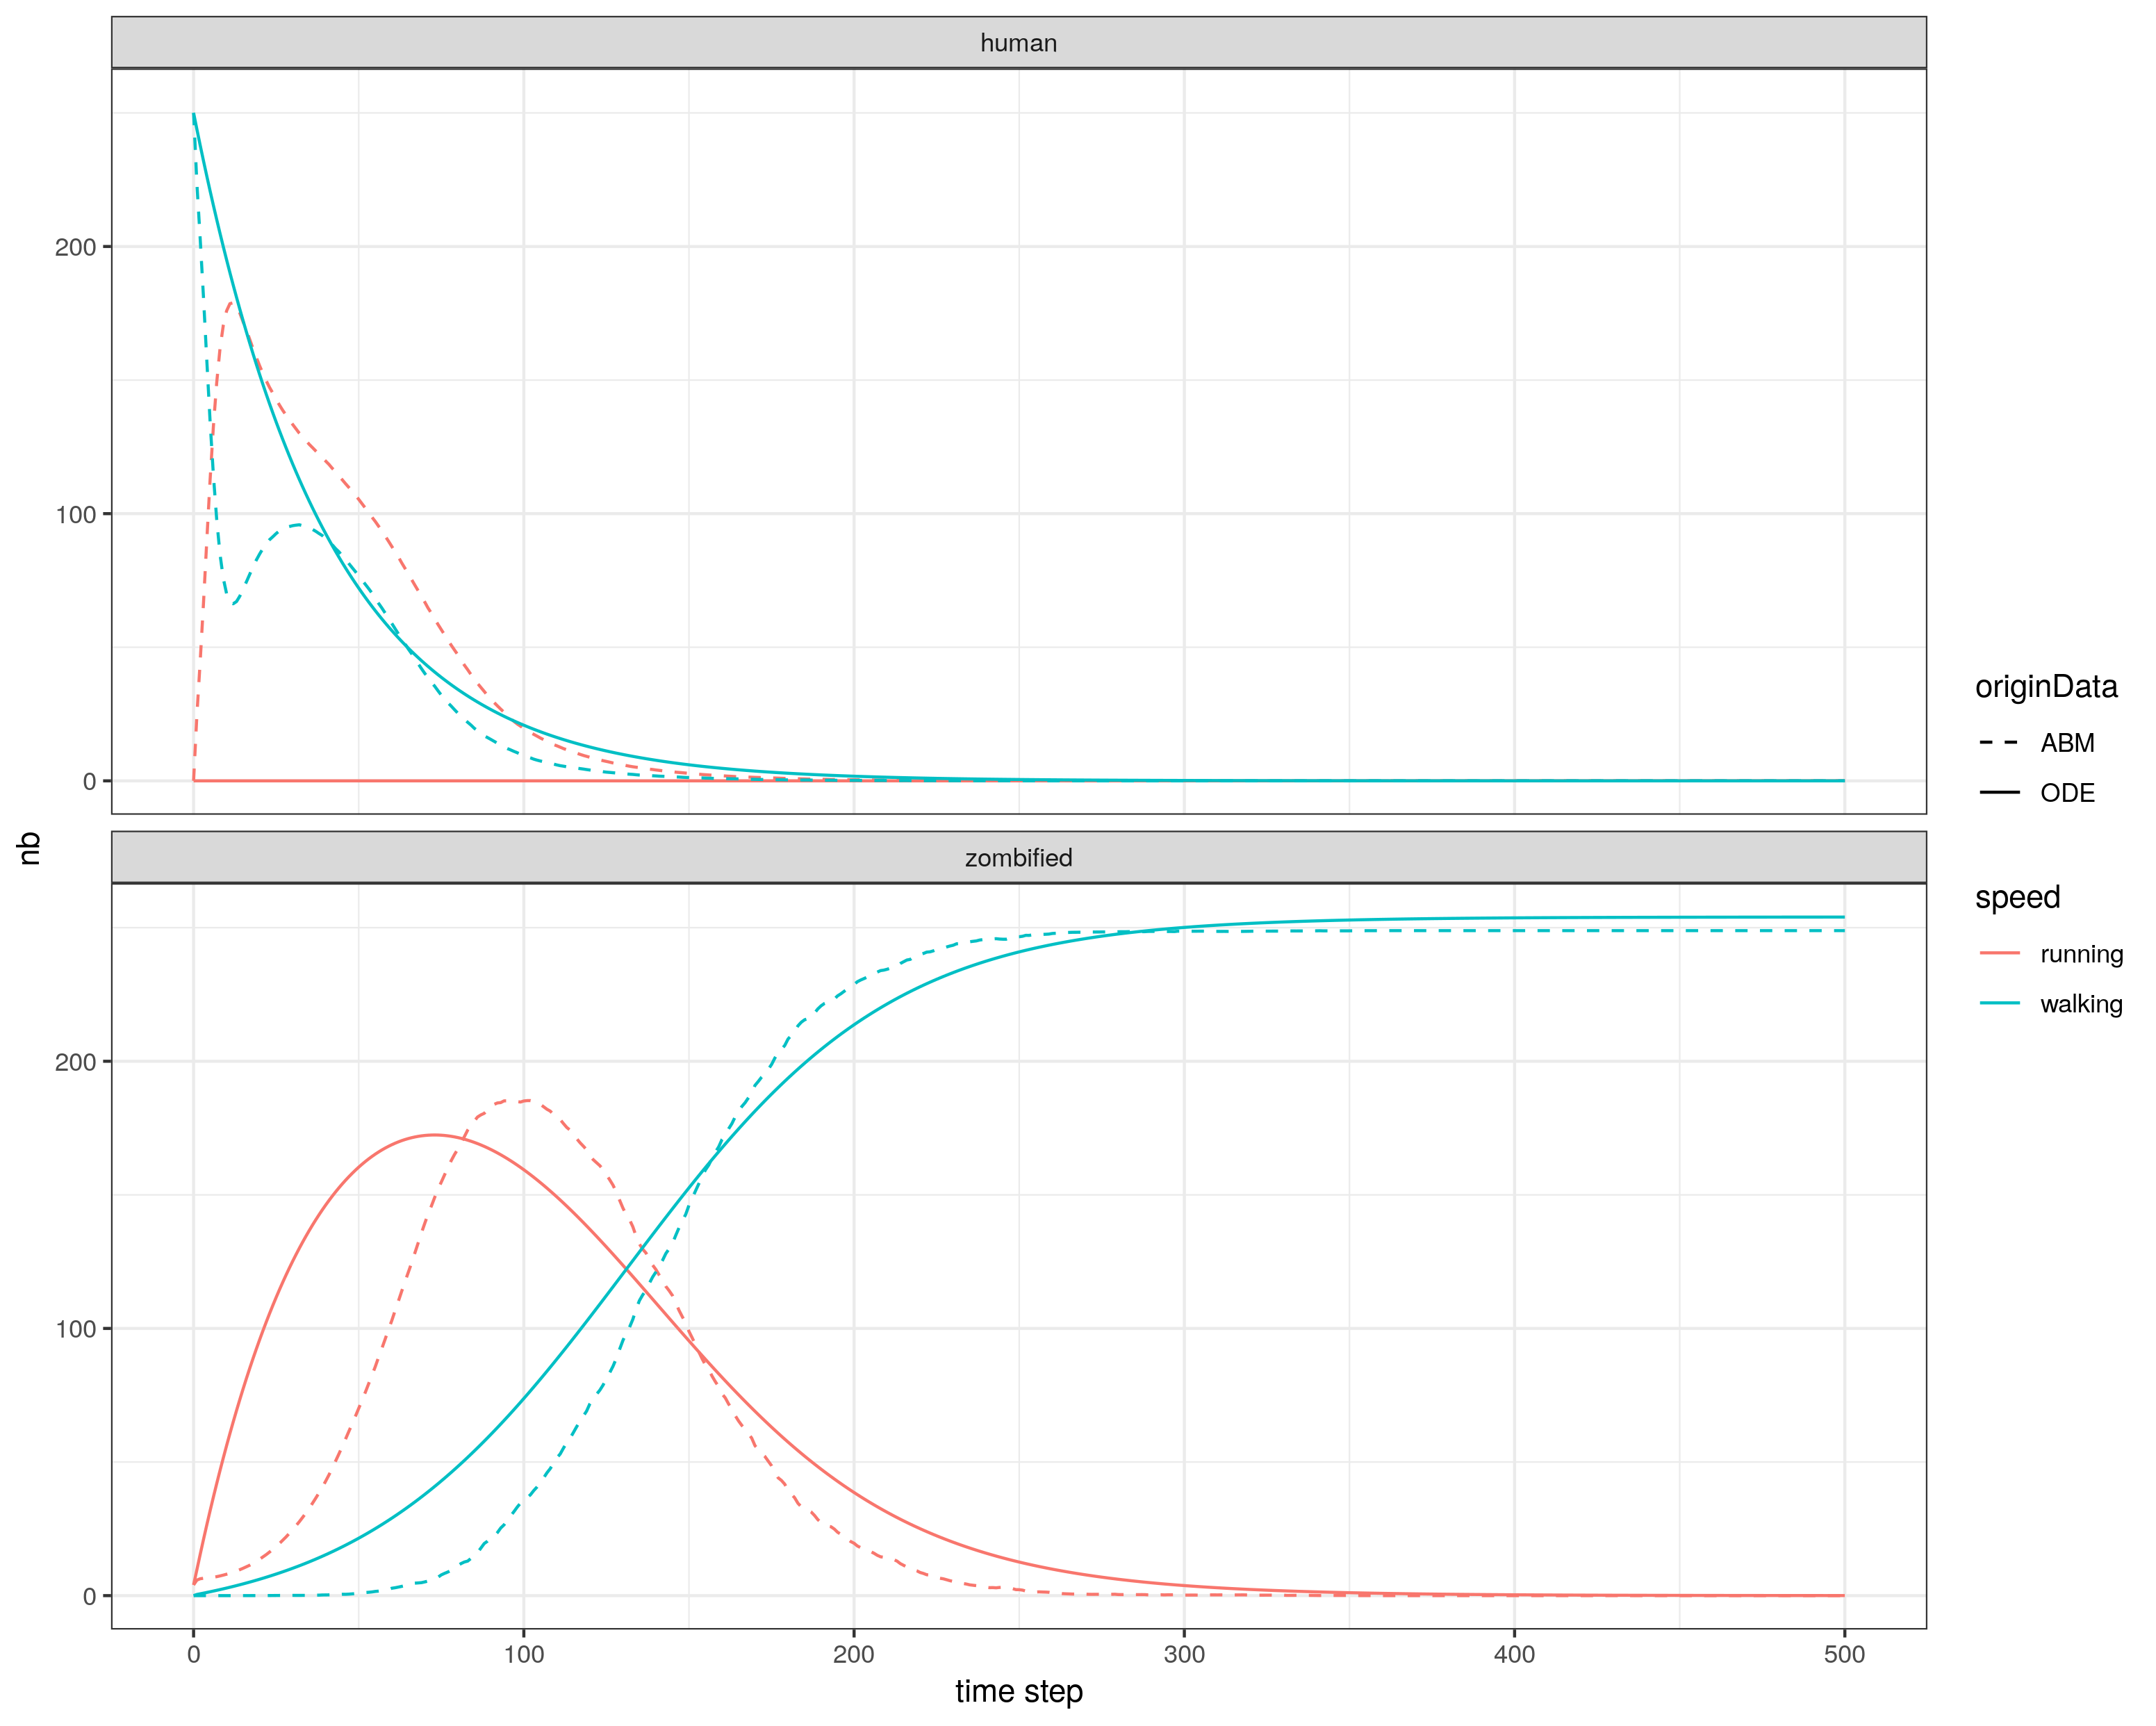
\includegraphics[width=\textwidth]{figures/parcimony/parcimony_dynamics_1.png}
}


\sframe{Dynamics for 2 mechanisms activated}{
	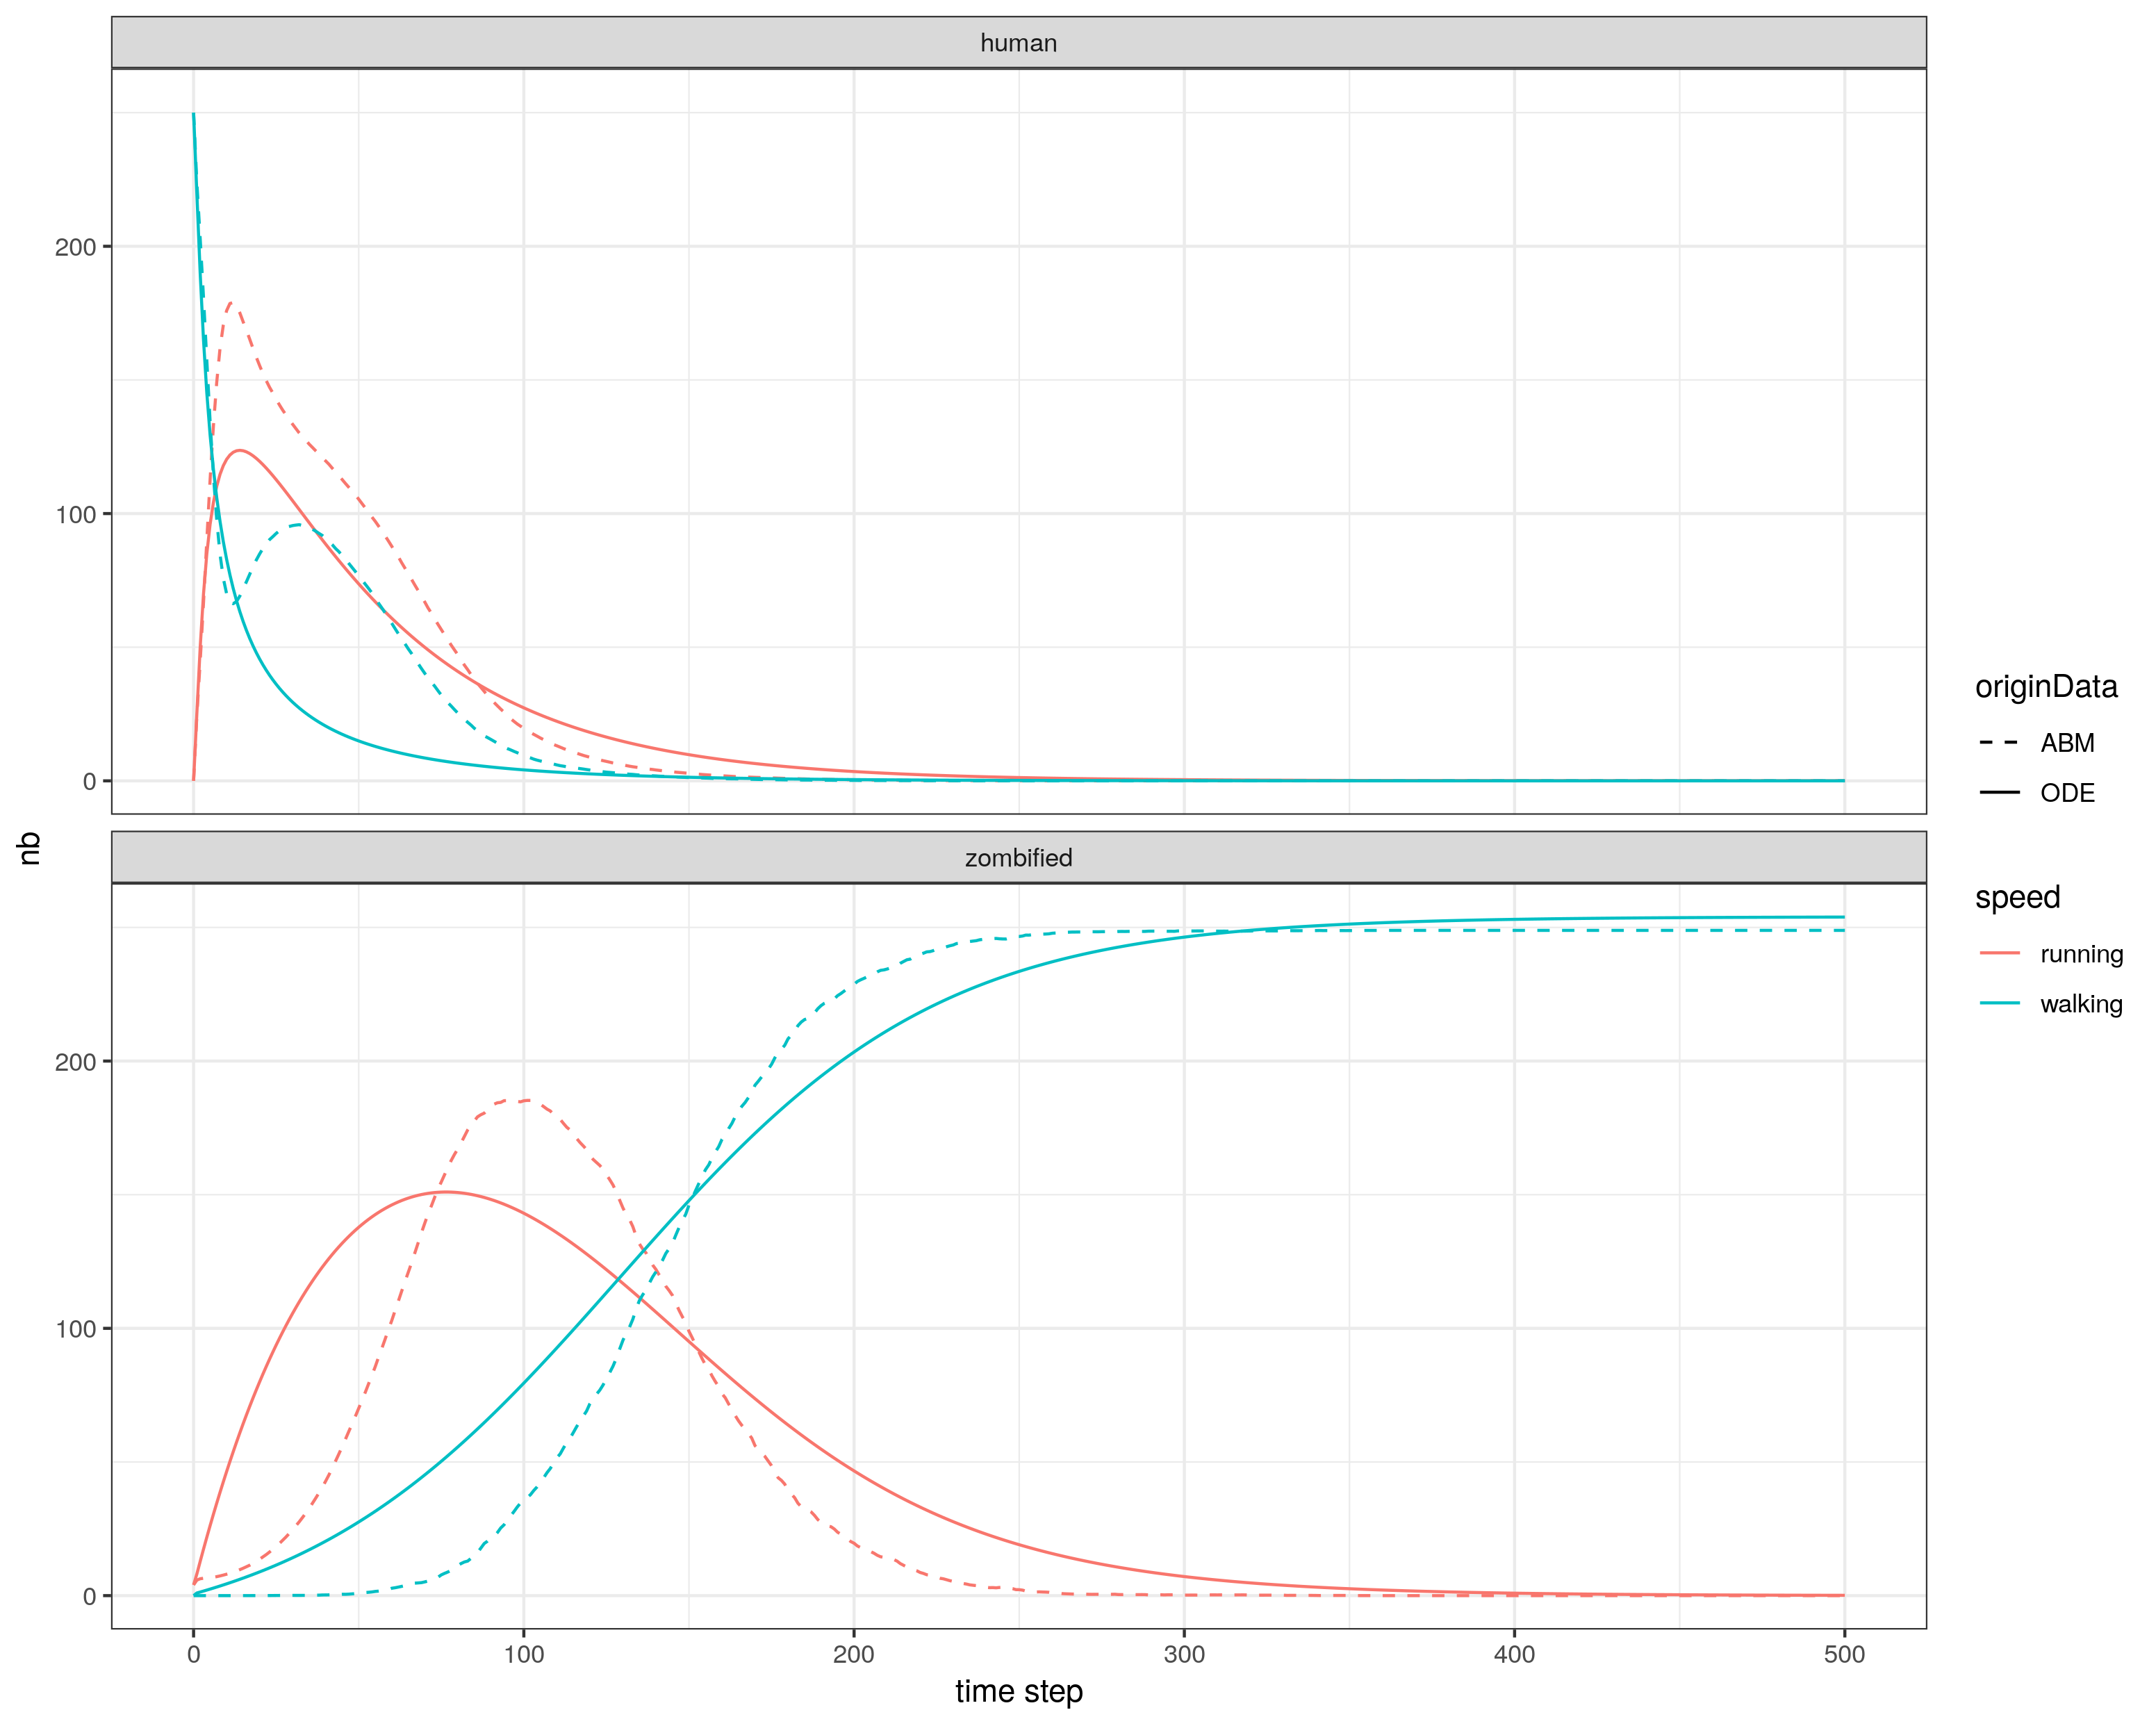
\includegraphics[width=\textwidth]{figures/parcimony/parcimony_dynamics_2.png}
}


\sframe{Dynamics for 3 mechanisms activated}{
	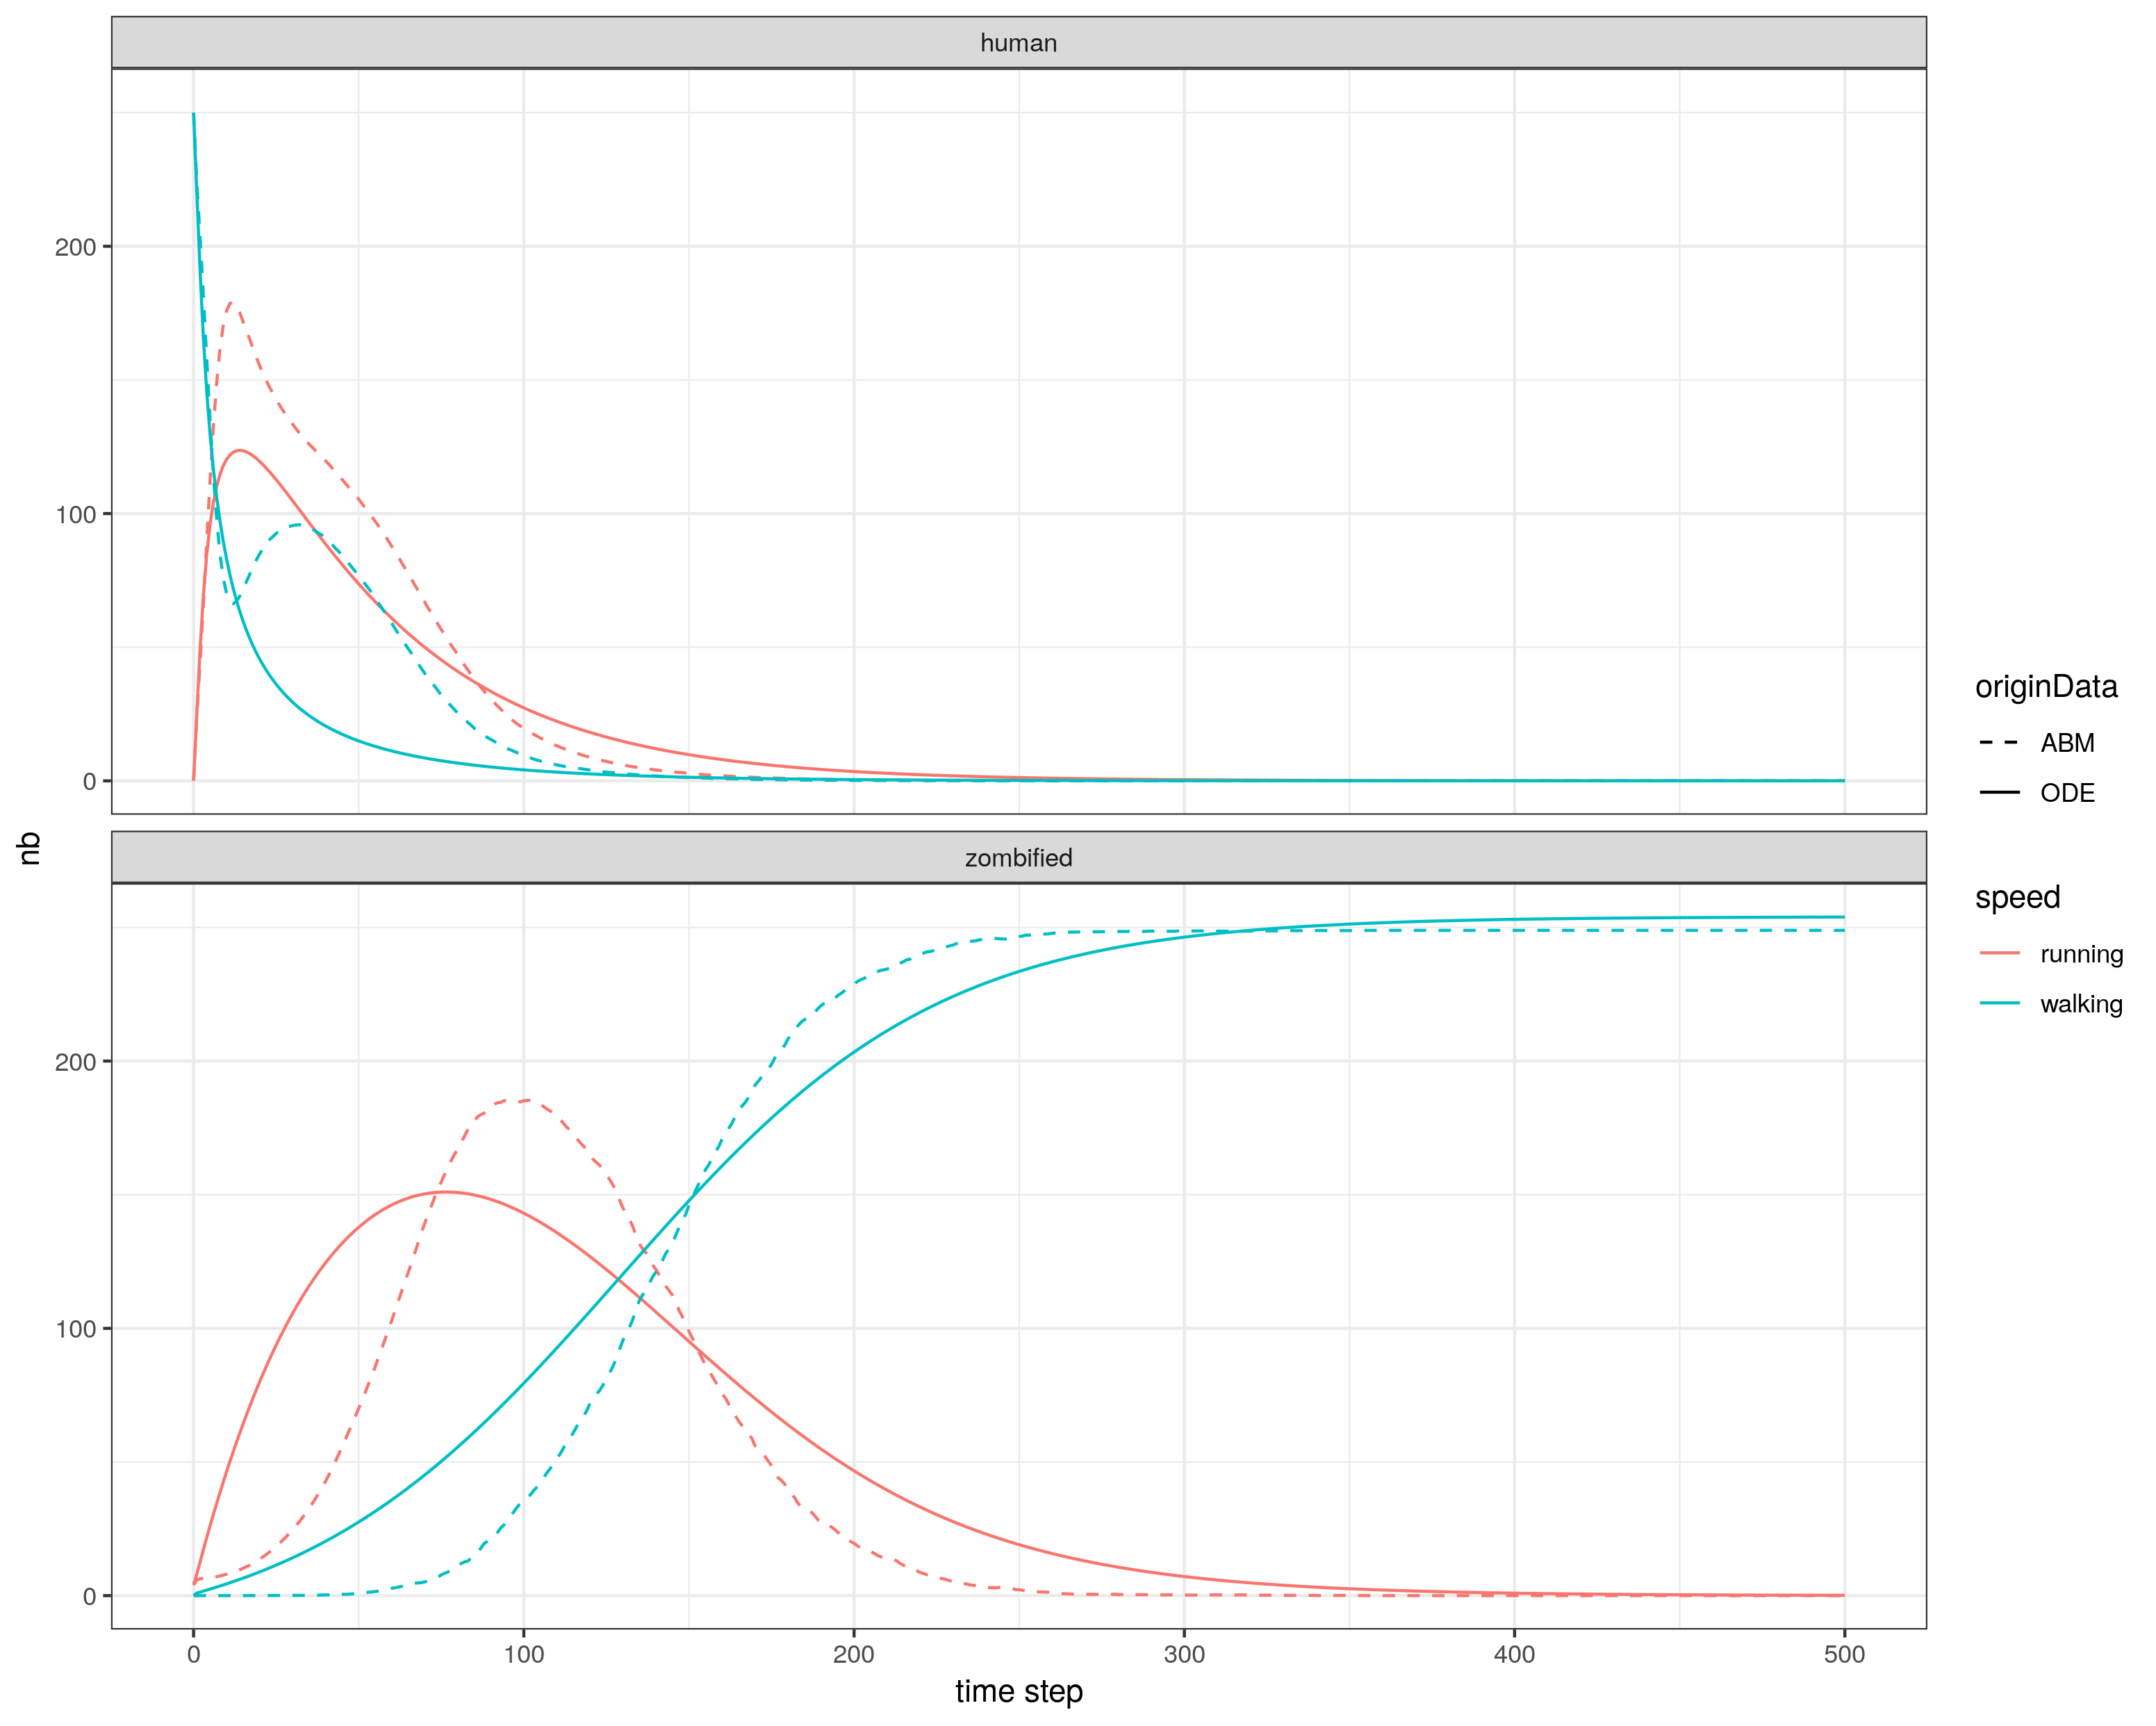
\includegraphics[width=\textwidth]{figures/parcimony/parcimony_dynamics_3.png}
}


\section{Some mathematics}

\sframe{A few math remarks}{
	Recall the ODE system:	
	
	\bigskip
			
\fontsize{8pt}{9pt}\selectfont
		$\left\{
		\begin{array}{lcl}
			\dv{H_{walk}}{t}  & = &  -(panic0 * \frac{Z_{walk}+Z_{run}}{N} + inf) * H_{walk} + exhaustH * H_{run}  \\
			\tmspace{1mu}&& \\
			\dv{H_{run}}{t} & = & panic0 * \frac{Z_{walk}+Z_{run}}{N} * H_{walk} - (exhaustH + inf) * H_{run} \\
			\tmspace{1mu}&& \\
			\dv{Z_{walk}}{t} & = & inf * (H_{walk} + H_{run}) - hunt0 * \frac{H_{walk}+H_{run}}{N} * Z_{walk} + exhaustZ * Z_{run} \\
			\tmspace{1mu}&& \\
			\dv{Z_{run}}{t} & = & hunt0 * \frac{H_{walk}+H_{run}}{N}* Z_{walk} - exhaustZ * Z_{run}
		\end{array}
		\right.
		$
%\normalsize
\bigskip
\bigskip

Where $N := H_{walk}+H_{run}+Z_{walk}+Z_{run}$

\bigskip
\normalsize
%
First-order \textbf{nonlinear} (autonomous) ordinary differential equation... a priori no explicit solution, hence numerical solutions.
%Equation différentielle \textbf{non linéaire} d'ordre 1... a priori on ne sait pas trouver de solutions explicites, d'où la résolution numérique

}




%\sframe{Cauchy Problem}{
%
%Let's note $X(t) :=  (H_{walk}(t),H_{run}(t),Z_{walk}(t),Z_{run}(t)) $
%
%We have the following Cauchy problem:
%
%$$ 
%\left\{
%\begin{array}{llll}
%X'(t) & = &  F(X(t)) & \\ 
%X(0) & = & (x_0,y_0,z_0,w_0) & \text{ initial condition}
%\end{array}
%\right.
%$$
%
%where  
%
%$$ (x_0,y_0,z_0,w_0)  \in \mathbb{R}_+^* $$
%
%and
%
%\fontsize{7pt}{8pt}\selectfont
%$$\begin{array}{lllll}
%F & : & \mathbb{R}^4 & \to     & \mathbb{R}^4 \\
%  &   &   (x,y,z,w)       &  \mapsto &  F(x,y,z,w) := ((panic0 * \frac{z+w}{x+y+z+w} + inf) * x + exhaustH * y,  \\
%  & & & &  \hspace{2cm} \ldots,\ldots,\ldots)
%\end{array}$$
%
%\normalsize
%Cauchy-Lipschitz theorem: Existence and uniqueness to a solution of the Cauchy problem.
%
%}




\sframe{Total population size}{

Summing the 4 equations, we have:

$$ \dv{N}{t} = \dv{H_{walk}}{t} + \dv{H_{run}}{t} + \dv{Z_{walk}}{t} + \dv{Z_{run}}{t} =0 $$

So $N(t)$ is constant:
$$ N(t) = N(0), \text{ for all } t.$$

We find back that the population size (human + zombies) is constant: natural !

}



\sframe{Human / zombies population size}{

Let's note $ H := H_{walk} + H_{run}$

Summing the first equations, we have:

$$ \dv{H}{t} = \dv{H_{walk}}{t} + \dv{H_{run}}{t}  = - inf * (H_{walk}(t) +H_{run}(t)) = - inf * H(t)$$

First-order linear ordinary differential equation with constant coefficient: explicit solution !
%Equation différentielle linéaire d'ordre 1 à coefficient constant pour $H$: on sait résoudre !

$$ H(t) = H(0) * e^{-inf *t} $$
 
Likewise, $$ Z(t) := Z_{walk} + Z_{run} = N - H(t) $$

}


\sframe{Equilibrium points}{


\textbf{Definition:} The point $x \in \mathbb{R}^4$ is an \textit{equilibrium point} for the differential equation $X' = F(X)$ if $F(X) = 0$.

\bigskip
\bigskip

For example, points of the form $(0,0,0,N)$ are equilibrium points. They correspond to a population composed of walking zombies.

}


\sframe{Link with Parcimony}{

Theses 2 facts : 

\begin{itemize}
\item $N(t)$ constant 
\item solutions for $H$  and  $Z$ 

... are still valid for the system with additional mechanism.

\bigskip
$\rightarrow$ Not able to change the shape of the solutions of the equation of $H$ and $Z$ with such system modifications.
\end{itemize}

}


%% Stop numbering
\backupbegin

\appendix

\backupend

\end{document}